\documentclass[UTF8,12pt,a4paper]{ctexart}
\usepackage{amsmath,amssymb,bm,mathtools}
\usepackage{booktabs,longtable,tabularx,array,multirow}
\usepackage{geometry,graphicx,float,caption,subcaption}
\usepackage{enumitem,fancyhdr,xcolor}
\usepackage[hidelinks]{hyperref}
\usepackage{fvextra}
\geometry{left=2.5cm,right=2.5cm,top=2.5cm,bottom=2.5cm}
\setlength{\parindent}{2em}
\setlength{\parskip}{0pt}
\linespread{1.18}
\captionsetup{font=small,labelsep=quad}
\pagestyle{fancy}
\fancyhf{}
\cfoot{\thepage}
\renewcommand{\headrulewidth}{0pt}
\newcommand{\keywords}[1]{\par\vspace{0.6em}\noindent\textbf{关键词：}#1}
\newcommand{\R}{\mathbb{R}}
\newcommand{\pos}[1]{\left(#1\right)^{+}}
\newcolumntype{Y}{>{\centering\arraybackslash}X}
\setmonofont{Consolas}

\title{考虑因果预测与日内调账的微网电力调控策略}
\author{}
\date{}

\begin{document}
\maketitle
\thispagestyle{plain}
\begin{abstract}
针对含光伏、负荷与储能的微网在日前购电、日内合同调整和变动电价下的协同调度问题，本文建立一套严格遵守信息发布时间的滚动优化框架。首先将附件中以区间终点标记的10分钟数据统一映射为自然时段，把功率换算为每槽电量，并以母线平衡、储能效率、功率上限和荷电状态约束构成统一物理层。问题一采用循环日线性规划，以购电费用为主目标、储能吞吐量为次目标，得到典型日购电量 $59482.6982\,\mathrm{kWh}$、费用 $35126.9489$ 元，且荷电状态由 $6000\,\mathrm{kWh}$ 出发并回到同一水平。

对于问题二，本文只使用决策时刻之前的历史数据：以90日以内相似日得到负荷和光伏点预测，以60日以内的负荷--光伏联合残差构造场景，再用边际经验分位数压缩为保守轨迹并求解线性规划。正式统计覆盖2025年2月至12月共334日，1月仅用于历史启动和储能状态连续推进。固定电价下，无日内调账策略的现金费用为 $18764165.93$ 元，应急购电为 $578081.54\,\mathrm{kWh}$。相似日负荷预测的 MAE 和 RMSE 分别为 $722.57$、$904.09\,\mathrm{kW}$；名义90\%经验区间的实际覆盖率仅为83.11\%，因此本文不把该区间解释为概率保证。

对于问题三，在0、6、12、18时接收官方光伏预测，并以最近60个已完成日期的同发布时刻误差作因果偏差修正，只重算尚未执行的合同。该策略费用为 $16279696.69$ 元、应急购电为 $115458.15\,\mathrm{kWh}$，较问题二节约 $2484469.24$ 元；这一差异同时包含信息改善与更新规则变化，不能全部归因于更新次数。进一步在相同0时信息下比较更新集合，基于最新官方预测和已观测前缀构造的2小时合成更新相对6小时方案节约 $708343.30$ 元，但在另一种合同结算解释下仅节约 $127065.26$ 元，说明建议依赖结算条款和更新成本。

对于问题四，未来电价预测只采用过去30日同槽中位数及当日已实现偏差，实际电价仅用于结算。无调账与有调账方案的现金费用分别为1925.45万元和1673.51万元，后者应急购电为 $115938.21\,\mathrm{kWh}$。变价条件下2小时方案相对6小时方案节约70.16万元；若每次额外更新成本高于约262.59元，则该增频不再具有净经济优势。通过54组基线与单因素实验、逐槽能量平衡、跨日储能连续性和未来信息扰动检验，验证了算法的数值可行性与因果性。本文方法实质上是边际分位轨迹驱动的滚动线性规划，适用于题设数据和结算假设，不等同于完整随机模型预测控制，也不提供样本外概率保证。

\keywords{微网调度；因果预测；滚动线性规划；经验分位数；储能；合同调账}
\end{abstract}
\clearpage
\setcounter{page}{2}
\section{问题重述与分析}

\subsection{问题背景与任务拆解}

微网由光伏电源、用电负荷、储能装置以及与外部电网相连的购电通道构成。光伏和负荷均具有显著的日内波动，且真实值在决策后才逐步显现；储能能够在时段之间转移电量，却受到容量、功率和往返损耗限制。若日前合同偏低，实时缺口必须以高倍率应急电价补齐；若合同偏高，多余合同电量又可能无法获得完全退款。因此，本题不是单纯的峰谷套利，而是预测误差、合同规则、储能状态和信息更新时间共同作用的序贯决策问题。

已有研究通常将微网不确定性表示为场景、随机过程或滚动预测控制问题\cite{liang2014survey,hu2021mpc}。两层随机模型预测控制可同时处理较慢的计划层与较快的反馈层\cite{raimondi2018twolayer}，日前市场和储能联合优化也常用随机规划刻画\cite{zhao2020dayahead}。滚动时域方法则在新信息到达时重求后续决策\cite{silvente2015rolling}。本题数据量有限，且需要输出指定时段的可核验合同、电池和应急购电结果。为此，本文采用“因果预测--分位轨迹--线性规划--实际执行”的透明结构：不假定未来真实量已知，不把复杂场景树直接塞入控制器，而是用历史联合残差估计风险，再压缩为一条可解释的保守轨迹。

四个问题形成逐层递进关系：
\begin{enumerate}[label=（\arabic*）]
  \item 问题一给出典型日负荷、光伏和固定电价，要求在日末恢复初始荷电状态。它用于确定物理约束、时间口径和确定性调度基线。
  \item 问题二将负荷和光伏扩展至全年，但不允许日内调整购电合同。核心是用历史构造次日预测和不确定性余量，并让储能状态跨日连续。
  \item 问题三在0、6、12、18时获得官方光伏预报，可对尚未执行的合同调账。核心是区分“当时已知信息”与“事后真实值”，并按题设规则只结算最终有效合同。
  \item 问题四把外部电网电价改为随时间变化，要求分别给出无调账和有调账策略。核心是对未来价格也实行因果预测，实际价格只在结算时使用。
\end{enumerate}

从决策目标看，本题至少包含三组相互牵制的量。第一组是合同费用与应急费用：增加日前合同会降低高价应急缺口，却可能产生更多闲置合同；第二组是供电可靠性与光伏消纳：保守净负荷有助于保障负荷，却可能挤占光伏在中午的消纳空间；第三组是当前收益与未来储能价值：过早放电能降低当前槽购电，但会增加后续高价槽的缺口。由此，本文不把单一电量或单一费用作为所有问题的评价标准，而是把现金费用作为优化目标，同时报告应急量、闲置合同、弃光和SOC末态，并用终端价值协调短期与后续时段。

问题间比较也需要统一合同。问题二与问题三使用相同固定电价和物理设备，问题四的两个方案使用相同变动电价序列；所有策略从1月1日同一SOC出发，2月至12月采用完全相同的统计日期。只有在这种共同基础上，费用差才具有可比性。另一方面，问题二到问题三不仅增加更新事件，也更换了光伏信息源，因此本文另设“相同0时信息”的0/12/6/2小时实验来分析更新集合；这一步避免把预报源变化误计为纯频率收益。

\subsection{信息集与评价口径}

令日期为 $d$，每天含 $T=144$ 个10分钟时槽，槽序号为 $t=0,1,\ldots,143$。在日期 $d$ 的事件时刻 $h$ 做决策时，可用信息集记为 $\mathcal F_{d,h}$。它包括：所有早于 $d$ 的完整日期数据、当天 $h$ 时之前已经实现的负荷与光伏、截至 $h$ 时已经发布的官方预报，以及变价情形下已经实现的价格。任何 $h$ 时之后的真实负荷、真实光伏和真实价格都不属于 $\mathcal F_{d,h}$。

为避免首月没有历史而导致模型断裂，计算从1月1日起推进；历史不足时用附件典型日收缩估计。储能状态从1月1日连续传递到12月31日，不在日界处重置。题目要求的结果统计期为2月1日至12月31日，共334日。因此，文中“年度费用”若无特别说明，均指这334日的正式统计，而原始年度负荷、光伏和价格分布图可使用365日数据。

评价指标包括现金费用、应急购电量、闲置合同电量、弃光量、储能末态和逐槽物理残差。预测部分报告 MAE、RMSE、MAPE及经验区间覆盖率，但MAPE仅在真实光伏大于 $100\,\mathrm{kW}$ 的样本上计算；若没有有效样本则记为缺失，而不是零误差。时间序列不是相互独立的重复实验，本文不使用未经验证的独立同分布显著性检验。

\subsection{总体建模流程}

模型首先将输入功率乘以 $\Delta t=1/6\,\mathrm h$ 得到时槽电量；随后基于 $\mathcal F_{d,h}$ 生成负荷、光伏和必要时的价格预测；再由历史联合残差计算经验场景及边际分位轨迹，求解满足储能约束的线性规划；最后用真实量在当前槽执行“余电充电、缺电放电、剩余缺口应急购电”的因果策略。新预报到达时，仅对尚未执行的合同段重复上述过程。典型日输入结构见图\ref{fig:q1-raw}。

这一流程保留了滚动优化的反馈结构，但与完整随机MPC不同：控制器输入的是压缩后的确定性分位轨迹，而非带联合概率的完整场景树。这样可以直接追溯每一项输出，同时也意味着经验区间和分位参数只反映本样本中的风险暴露，不能被解释为严格的机会约束保证。

\begin{figure}[H]
  \centering
  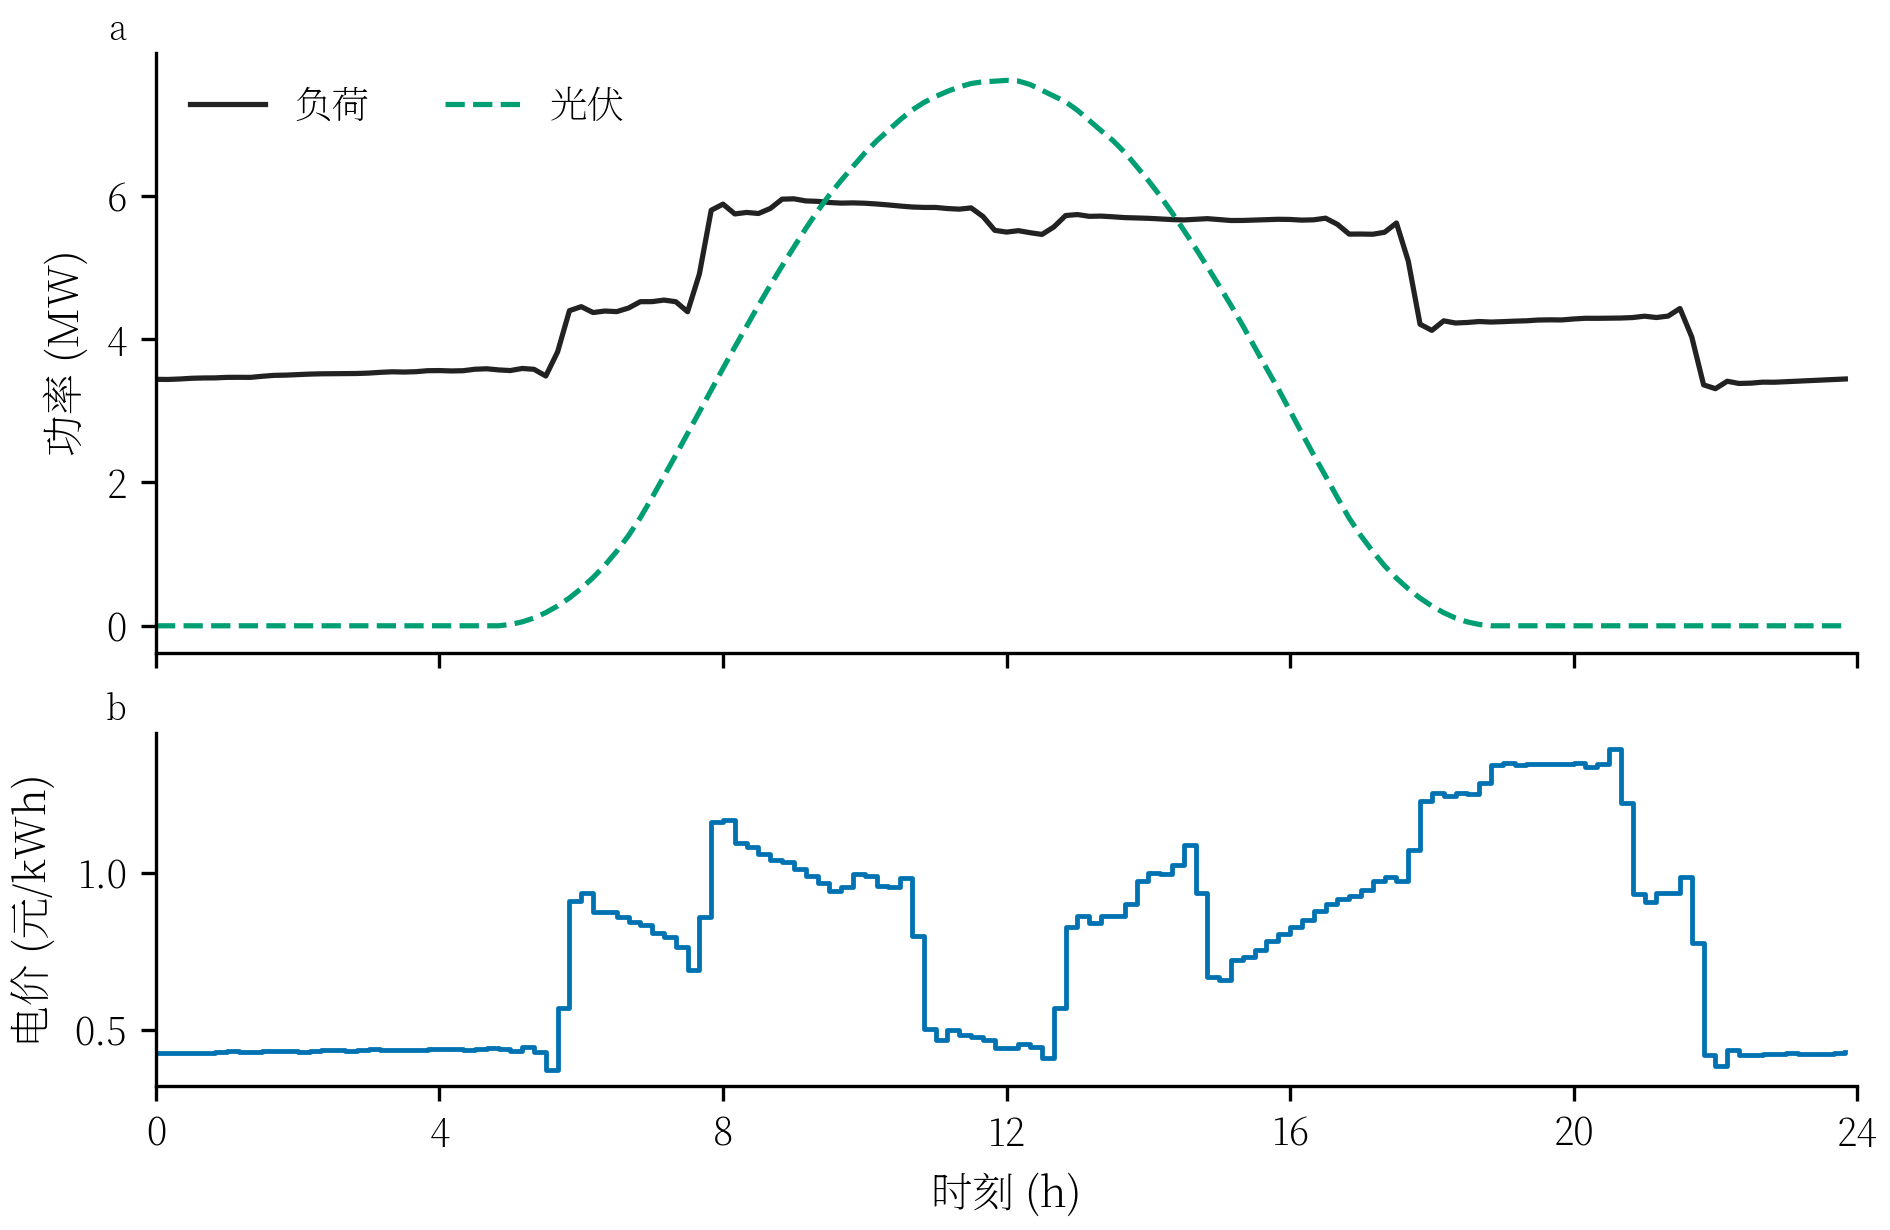
\includegraphics[width=0.96\textwidth]{figs/raw_q1_typical_profiles.png}
  \caption{典型日负荷、光伏与固定电价的日内结构。负荷和光伏峰值并不完全同步，电价阶梯又改变了储能转移能量的价值。}
  \label{fig:q1-raw}
\end{figure}

\section{模型假设、时间口径与符号}

\subsection{基本假设}

在不改变题面物理含义的前提下作如下假设：
\begin{enumerate}[label=（\arabic*）]
  \item 微网不能向外部电网反向售电。光伏可被负荷利用、用于充电或弃光；合同电量未使用的部分记为闲置合同电量。
  \item 储能容量为 $12000\,\mathrm{kWh}$，荷电状态限定在10\%至90\%，即 $1200\le S\le10800\,\mathrm{kWh}$；充、放电功率上限均为 $5000\,\mathrm{kW}$，单向效率均为0.9。
  \item 同一10分钟槽不主动同时充电和放电。线性规划若出现数值层面的极小共存量，在执行和审计时按容差处理；真实结果未出现有意义的同时充放。
  \item 问题一为循环典型日，日末荷电状态等于日初；问题二至四按全年顺序推进，不施加每日循环约束。规划末端价值只用于抑制短视放电，不从报告的现金费用中扣除。
  \item 相似日、残差、偏差和价格预测均只能使用当前决策时刻以前可得的数据。官方光伏预报按其发布时刻进入信息集，跨年不可得的目标不参与误差计算。
  \item 题设未给出设备启停、老化、备用容量和配电网潮流限制，因此主目标只计外购合同及应急费用。储能吞吐量作为同费用解之间的次级筛选量，而不是虚构的货币成本。
\end{enumerate}

\subsection{10分钟时间映射}

附件中的时刻标签从00:10持续到24:00。本文将标签解释为自然10分钟区间的终点：00:10对应00:00--00:10，24:00对应23:50--24:00。设原始功率为 $P_t$，则时槽电量为
\begin{equation}
 E_t=P_t\Delta t,\qquad \Delta t=\frac16\ \mathrm h .
 \label{eq:power-energy}
\end{equation}
题面给出的Excel模板表头保持不变，数值按槽位置写入；论文中的指定时段、SOC边界点和聚合量统一采用自然区间。这一约定可同时避免把10分钟电量误作整小时电量，以及把24:00错误解释为下一日首槽。

\subsection{统一物理模型}

对任意日期和时槽，定义负荷电量 $L_t$、可用光伏电量 $V_t$、合同购电 $g_t$、闲置合同 $w_t$、光伏利用 $v_t$、充电 $x_t$、放电 $y_t$、应急购电 $u_t$ 和槽初荷电状态 $S_t$。母线平衡为
\begin{equation}
 g_t-w_t+v_t+y_t+u_t=L_t+x_t .
 \label{eq:balance}
\end{equation}
储能状态递推为
\begin{equation}
 S_{t+1}=S_t+\eta_c x_t-\frac{y_t}{\eta_d},
 \qquad \eta_c=\eta_d=0.9 .
 \label{eq:soc}
\end{equation}
约束写为
\begin{align}
 0\le v_t\le V_t,\quad &0\le w_t\le g_t, \label{eq:renew}\\
 0\le x_t\le P_{\max}\Delta t,\quad &0\le y_t\le P_{\max}\Delta t, \label{eq:power}\\
 S_{\min}\le S_t\le S_{\max},\quad &u_t\ge0. \label{eq:bounds}
\end{align}
其中 $P_{\max}\Delta t=833.3333\,\mathrm{kWh}$。等式\eqref{eq:balance}把“合同已购买但未使用”的 $w_t$ 明确列出，因而合同电量、实际供能和现金费用不会混淆；式\eqref{eq:soc}在充放电两侧分别计入效率，往返效率为 $0.81$。

\subsection{主要符号}

全文主要符号、单位和决策角色汇总于表\ref{tab:symbols}。特别地，功率变量只在输入和图中使用kW，进入优化器后统一乘以时长成为kWh；SOC也是kWh，因而式\eqref{eq:balance}和式\eqref{eq:soc}两侧量纲一致。价格乘以合同或应急电量后得到元。这个转换看似简单，却决定了5000 kW功率上限在单槽中应为833.3333 kWh，而不是5000 kWh。

\begin{table}[H]
\centering
\caption{主要符号及单位}
\label{tab:symbols}
\begin{tabularx}{\textwidth}{c c X}
\toprule
符号 & 单位 & 含义\\
\midrule
$d,t,h$ & -- & 日期、10分钟时槽、预报或调账发布时刻\\
$L_t,V_t$ & kWh & 时槽负荷电量、可用光伏电量\\
$g_t,w_t$ & kWh & 合同购电量、闲置合同电量\\
$v_t,x_t,y_t,u_t$ & kWh & 光伏利用、充电、放电、应急购电\\
$S_t$ & kWh & 时槽初荷电状态\\
$c_t$ & 元/kWh & 外部电网基准价格或实际价格\\
$p_t,q_t$ & kWh & 0时不可变基准合同、最终有效合同\\
$\alpha$ & -- & 保守净负荷经验分位水平，主方案固定为0.8\\
$\mathcal F_{d,h}$ & -- & 日期$d$在时刻$h$可获得的信息集\\
\bottomrule
\end{tabularx}
\end{table}

式\eqref{eq:balance}还区分了合同购电 $g_t$ 与真正流入微网的 $g_t-w_t$。如果省略 $w_t$，当合同供给超过负荷、充电能力和光伏消纳需求时，模型要么被迫虚构用电，要么错误允许向外送电。显式设置闲置合同变量后，过购不会破坏能量平衡，同时仍按合同规则计费。类似地，弃光量为 $V_t-v_t$，它与闲置合同来自不同能源侧，二者不能合并为一个“浪费”变量。

对于全年策略，日末SOC不是固定参数，而是下一日的日初状态。设第$d$日末为 $S_{d,144}$，则连接条件为
\begin{equation}
 S_{d+1,0}=S_{d,144}.
 \label{eq:day-link}
\end{equation}
这一约束使1月的预测和调度虽然不进入正式费用统计，却仍会通过SOC影响2月1日。若每天强行重置到6000 kWh，相当于在午夜无成本注入或抽走能量，会系统性扭曲年度费用。

\section{问题一：典型日循环优化}

\subsection{确定性线性规划}

问题一的负荷、光伏和电价均已知，且不允许应急购电。令购电价格为 $c_t$，主目标为
\begin{equation}
 \min\ C_1=\sum_{t=0}^{143}c_tg_t,
 \label{eq:q1objective}
\end{equation}
并在式\eqref{eq:balance}--\eqref{eq:bounds}基础上增加 $u_t=0$、$S_0=S_{144}=6000$。该模型是线性规划。由于同一最优费用下可能存在多种等价储能轨迹，先求得最小费用 $C_1^*$，再在
\begin{equation}
 C_1\le C_1^*+10^{-8}\max\{1,|C_1^*|\}
 \label{eq:q1tol}
\end{equation}
的容差内最小化 $\sum_t(x_t+y_t)$。因此，报告的费用具有主目标最优性，而储能轨迹是低吞吐代表解，不宣称是唯一最优轨迹。

\subsection{调度结果}

求解得到总购电量 $59482.698167\,\mathrm{kWh}$，现金费用 $35126.948941$ 元；全天充电量和放电量分别为 $20740.661758$ 与 $16799.936024\,\mathrm{kWh}$，弃光为0。初末SOC均为 $6000\,\mathrm{kWh}$，全天最小与最大SOC恰为 $1200$ 和 $10800\,\mathrm{kWh}$。逐槽母线平衡最大绝对残差为 $9.10\times10^{-13}\,\mathrm{kWh}$。

图\ref{fig:q1-schedule}显示储能在低价时段吸收外购电或光伏，在高价时段放电。由于单向效率为0.9，只有足够大的价差才能覆盖往返损耗；约束边界处的平段说明容量而非价格判断成为局部瓶颈。日末恢复6000 kWh保证该典型日策略不通过透支期末电量来虚降费用。

\begin{figure}[H]
  \centering
  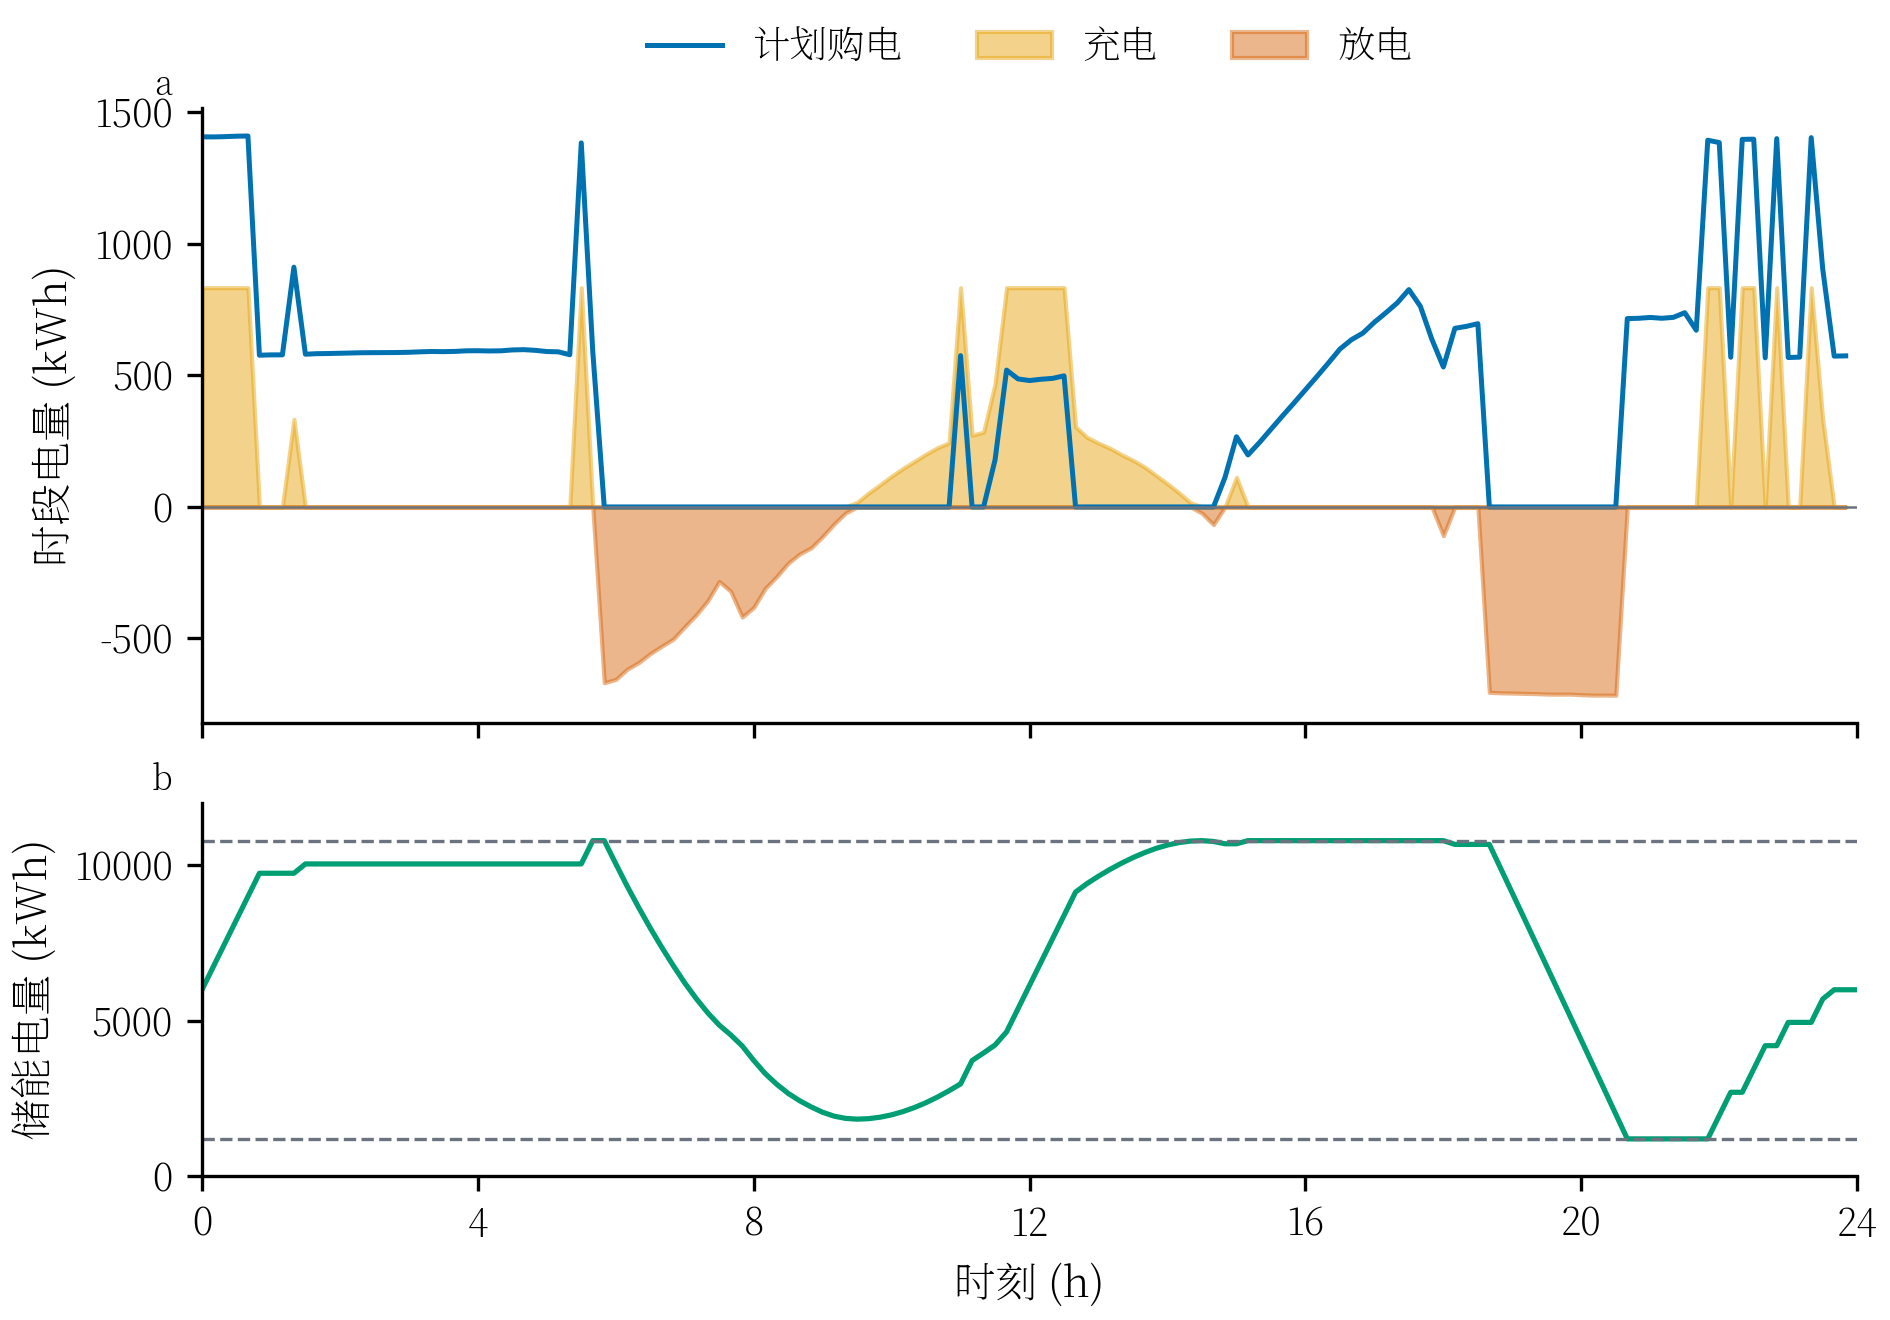
\includegraphics[width=0.97\textwidth]{figs/result_q1_optimal_schedule.png}
  \caption{问题一最优购电、充放电与SOC轨迹。SOC序列含0时和24时两个边界点。}
  \label{fig:q1-schedule}
\end{figure}

题目指定的六个10分钟购电量列于表\ref{tab:q1purchase}。其中12:00、16:00和18:00时起始槽需要购电，而10:00、14:00和20:00时起始槽购电为0。这里每个数值对应单个10分钟槽，不是整小时电量。

\begin{table}[H]
\centering
\caption{问题一指定时段购电量}
\label{tab:q1purchase}
\resizebox{\textwidth}{!}{%
\begin{tabular}{ccccccc}
\toprule
自然区间 & 10:00--10:10 & 12:00--12:10 & 14:00--14:10 & 16:00--16:10 & 18:00--18:10 & 20:00--20:10\\
\midrule
购电量/kWh & 0 & 480.41245 & 0 & 445.43165 & 531.89405 & 0\\
\bottomrule
\end{tabular}}
\end{table}

四小时聚合结果见表\ref{tab:q1battery}。充电量和放电量均由对应24个10分钟槽求和，SOC则取自然0时和24时边界。

\begin{table}[H]
\centering
\caption{问题一各4小时储能电量}
\label{tab:q1battery}
\begin{tabular}{crr@{\qquad}crr}
\toprule
时段 & 充电/kWh & 放电/kWh & 时段 & 充电/kWh & 放电/kWh\\
\midrule
0--4时 & 4500.000 & 0.000 & 12--16时 & 5286.035 & 91.101\\
4--8时 & 833.333 & 6365.838 & 16--20时 & 0.000 & 5780.132\\
8--12时 & 4787.960 & 1702.997 & 20--24时 & 5333.333 & 2859.868\\
\midrule
\multicolumn{3}{c}{0时SOC：6000 kWh} & \multicolumn{3}{c}{24时SOC：6000 kWh}\\
\bottomrule
\end{tabular}
\end{table}

若把全部标签整体解释为区间起点并循环平移10分钟，购电量几乎不变，而费用变为 $35126.848941$ 元，比主口径低约0.10元。这说明时间映射对总量稳健，但费用并非严格不变，故仍应统一自然区间定义。

\section{问题二：无日内调账的因果分位轨迹优化}

\subsection{滚动相似日预测}

问题二要求在每天开始前一次性确定全天合同，因而预测只能由过去日期生成。对目标日$d$，取最近90日内的历史日期集合 $\mathcal H_d$。对负荷，目标日与历史日星期属性相同时附加权重2，否则权重1；光伏不使用星期加权。时间衰减统一为
\begin{equation}
 \omega_{dk}=a_{dk}\exp\!\left(-\frac{d-k}{60}\right),\qquad k\in\mathcal H_d,
 \label{eq:analogweight}
\end{equation}
其中 $a_{dk}=2$ 或1。历史样本较少时，将加权历史均值向附件典型日收缩。以负荷为例，
\begin{equation}
 \widehat L_{d,t}=\gamma_d
 \frac{\sum_{k\in\mathcal H_d}\omega_{dk}L_{k,t}}
 {\sum_{k\in\mathcal H_d}\omega_{dk}}
 +(1-\gamma_d)L_t^{\mathrm{typ}},
 \qquad \gamma_d=\min\left(1,\frac{|\mathcal H_d|}{21}\right).
 \label{eq:analog}
\end{equation}
首日没有历史时直接采用典型日；光伏采用相同结构但 $a_{dk}=1$。该收缩使冷启动平滑过渡到滚动历史估计，不需要把未来全年样本先用于训练。

图\ref{fig:q2-raw}展示365日净负荷 $P_{\mathrm{load}}-P_{\mathrm{pv}}$ 的季节和日内结构。正负区间交替说明光伏富余与负荷缺口都具有显著时变性；仅用单个年度均值无法形成可执行合同。

\begin{figure}[H]
  \centering
  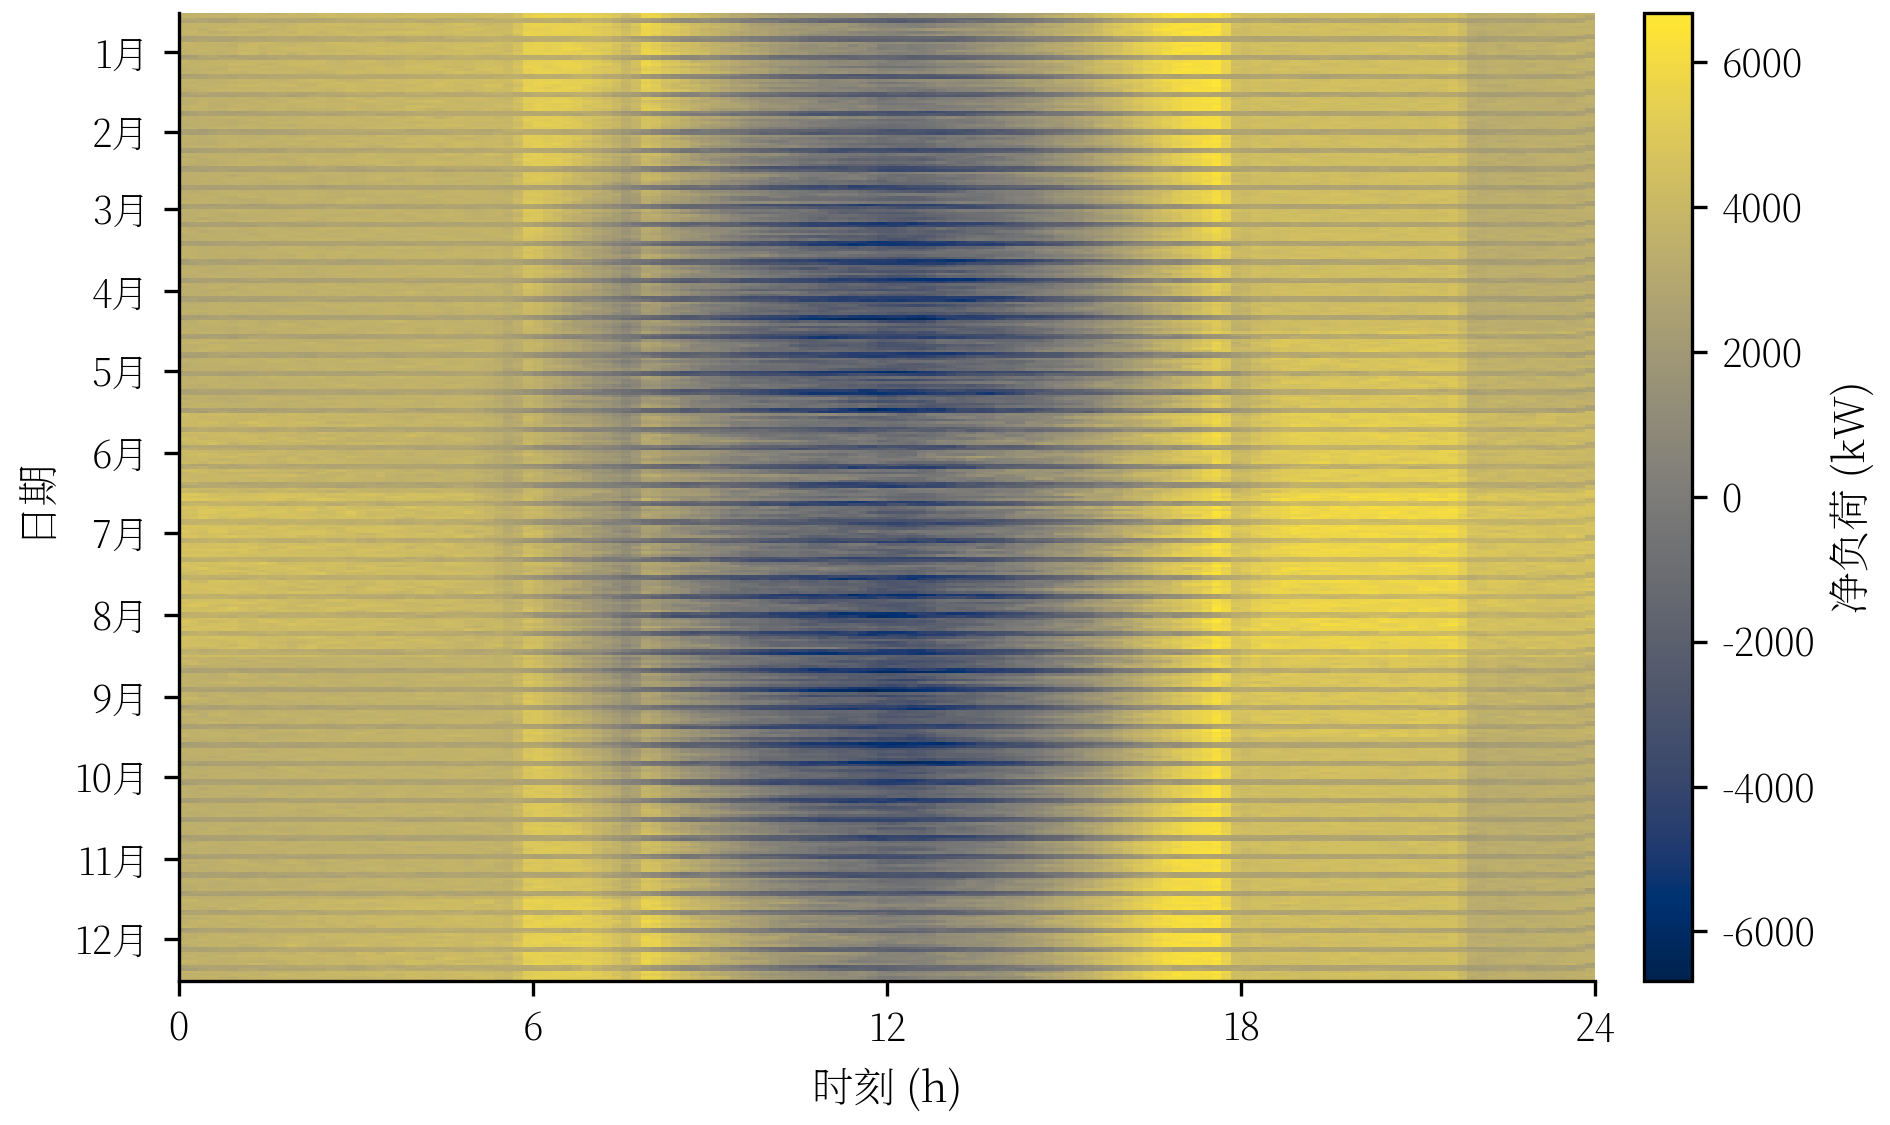
\includegraphics[width=0.98\textwidth]{figs/raw_q2_annual_netload.png}
  \caption{2025年365日净负荷的季节--日内分布。该图使用全年原始数据，策略费用统计期另为2月至12月。}
  \label{fig:q2-raw}
\end{figure}

在正式统计期上，相似日负荷预测 MAE 为 $722.5708\,\mathrm{kW}$，RMSE 为 $904.0899\,\mathrm{kW}$；光伏预测 MAE 为 $335.9217\,\mathrm{kW}$。图\ref{fig:q2-forecast}表明多数点接近45度线，但仍存在明显尾部误差。因此，单纯把点预测当作确定真值会低估应急购电风险。

\begin{figure}[H]
  \centering
  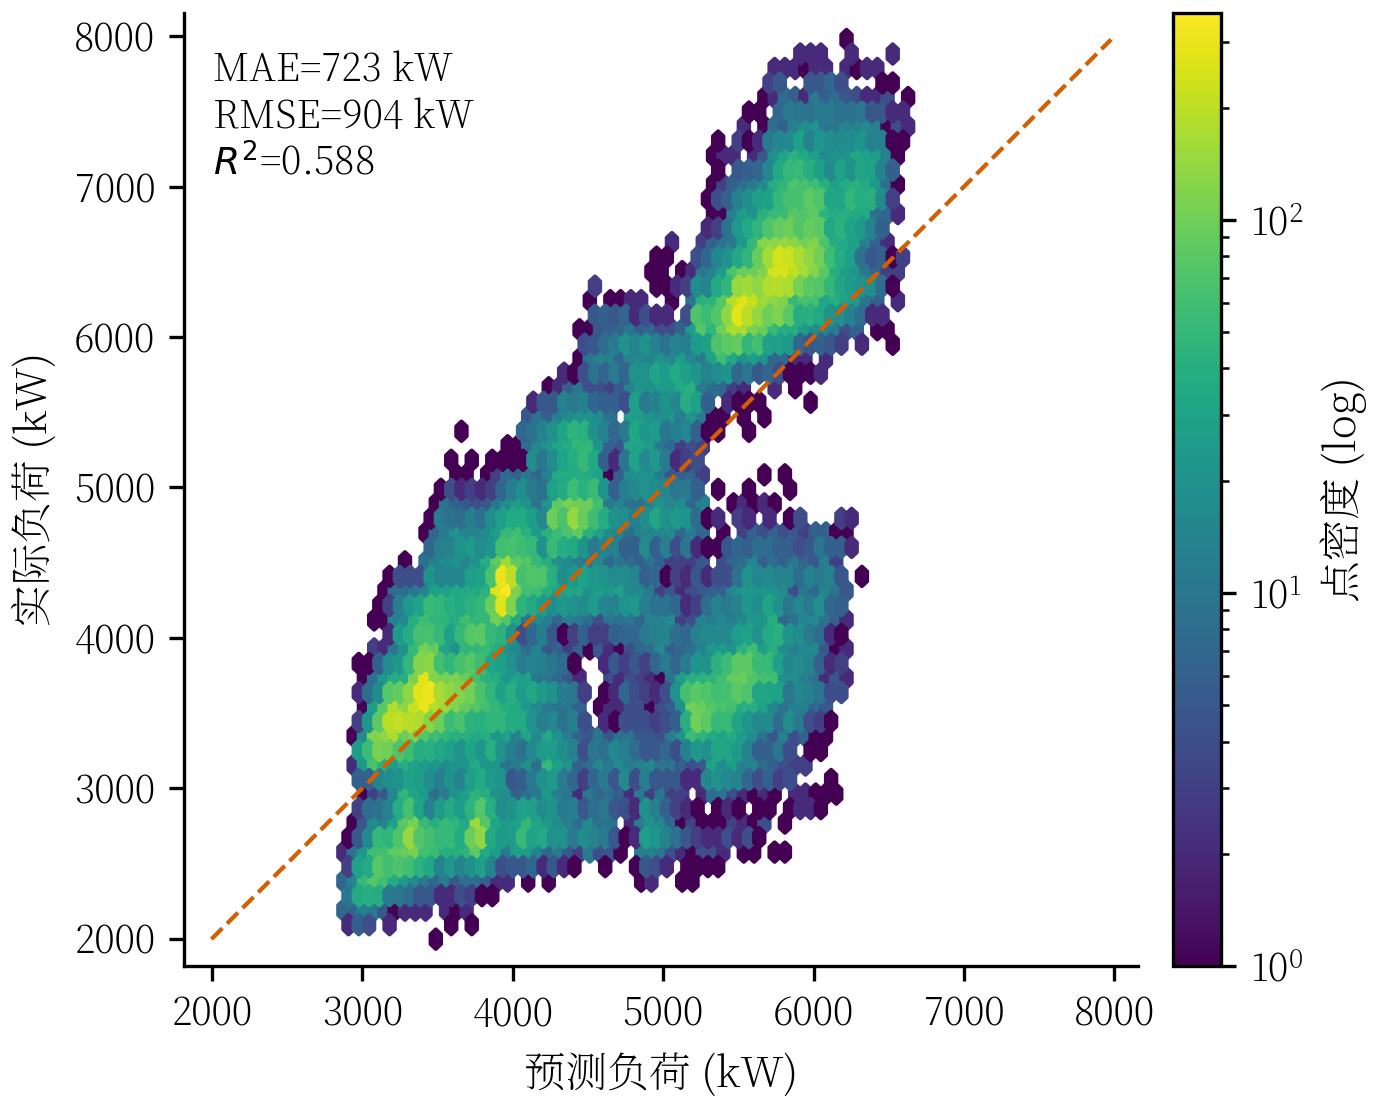
\includegraphics[width=0.72\textwidth]{figs/process_q2_forecast_validation.png}
  \caption{2月至12月因果相似日负荷预测与真实负荷的比较。颜色表示样本密度，离45度线较远的点对应尾部误差。}
  \label{fig:q2-forecast}
\end{figure}

\subsection{联合残差场景与边际分位压缩}

定义负荷和光伏残差
\begin{equation}
 e^{L}_{d,t}=L_{d,t}-\widehat L_{d,t},\qquad
 e^{V}_{d,t}=V_{d,t}-\widehat V_{d,t}.
 \label{eq:residual}
\end{equation}
在日期$d$只取最近60个已完成日期的残差，将一天的两类残差拼接为288维向量，并按各维历史标准差标准化。标准差小于 $10^{-9}$ 时置为1，避免近常数维放大数值误差。随后用 $K$-means 将残差日聚为至多9类，随机种子固定为2026，重复初始化10次；实际簇数不超过历史样本中唯一残差向量数。空历史退化为一个零残差场景，单条历史保留该样本本身。

设第$s$个场景的负荷和光伏轨迹为 $L^{(s)}_t,V^{(s)}_t$，簇权重为 $\pi_s$。对净负荷 $N^{(s)}_t=L^{(s)}_t-V^{(s)}_t$ 取加权经验 $\alpha$ 分位数，对光伏取 $1-\alpha$ 分位数：
\begin{align}
 \widetilde N_t &= Q_{\alpha}\!\left(\{N^{(s)}_t,\pi_s\}\right),\\
 \widetilde V_t &= \max\left\{Q_{1-\alpha}\!\left(\{V^{(s)}_t,\pi_s\}\right),-\widetilde N_t,0\right\},\\
 \widetilde L_t &= \widetilde V_t+\widetilde N_t.
 \label{eq:safe-trajectory}
\end{align}
经验分位数采用累计权重首次达到阈值的样本，不作线性插值。主方案在计算前固定 $\alpha=0.8$。式\eqref{eq:safe-trajectory}分别保守化净负荷和光伏，并通过重构保证 $\widetilde L_t,\widetilde V_t\ge0$ 及二者净差一致。

这种压缩保留了“净需求偏高、可用光伏偏低”的风险方向，却不再保留完整的跨时段联合分布。因此，后续优化应称为边际分位轨迹线性规划，而不是完整随机MPC。滚动残差给出的名义90\%经验区间对负荷、光伏的实际覆盖率分别为83.1109\%和83.4581\%，均低于90\%；它只能作为历史回测描述，不能构成概率保证。

从实现顺序看，每个日期的预测与规划包含五个确定步骤。首先读取不超过当前日期的历史索引，并生成相似日点预测；其次在历史残差上进行退化检查和标准化；再次聚类得到代表残差与经验权重；随后按式\eqref{eq:safe-trajectory}逐槽取分位数并重构安全负荷；最后以当天实际SOC为初态求解144槽LP。当天结束后才把真实残差加入下一日历史。该顺序保证“先预测、后观察、再更新历史”，不会因为一次性载入全年附件就把未来行用于当前决策。

选择边际分位压缩而没有直接对所有场景逐一设置供电约束，主要基于两点。其一，题目要求连续运行334个正式日期并完成54组实验，压缩后每次规划规模固定，便于稳定求解和逐槽复核；其二，分位参数 $\alpha$ 直接对应净负荷上侧与光伏下侧的保守方向，能够通过敏感性曲线解释风险偏好。代价是场景之间的时序相关只用于形成代表样本，进入LP后被一条轨迹替代。因此，本文把场景聚类视为风险特征提取，而非声称求解了多阶段随机规划。

\subsection{日前合同优化与真实执行}

在日期$d$的0时，用安全轨迹 $(\widetilde L_t,\widetilde V_t)$ 代替未知真实轨迹，求解统一物理模型。固定电价下，规划目标写为
\begin{equation}
 \min\ \sum_{t=0}^{143}c_tg_t-\lambda_d S_{144},
 \qquad \lambda_d=\eta_d\operatorname{median}\{c_t:t\text{属于剩余规划域}\}.
 \label{eq:q2plan}
\end{equation}
末端价值 $\lambda_d S_{144}$ 防止算法在一天末尾无代价地放空电池，但报告现金费用时不扣除这项信用。优化完成后合同 $g_t$ 全天不再改变。

真实槽到达时，执行层只使用当前真实负荷和光伏。若光伏及合同供给有余量，则先在功率和SOC允许范围内充电，之后的合同剩余计为闲置合同，光伏剩余计为弃光；若有缺口，则先放电，仍不能满足的部分以5倍当前电价应急购电。这个优先级是透明的因果反馈规则，而不是用全天真实量重新优化。

规划层与执行层分离有一个重要含义：LP给出的充放电计划服务于安全轨迹，真实执行动作则必须服从已实现的供需和当前SOC。若真实光伏高于保守轨迹，额外余电优先充电；若真实负荷高于轨迹，电池可能比计划更早放电。因而“计划合同总量”与“实际购电供能量”不完全相同，现金费用也不能由计划目标值直接替代，必须逐槽按真实执行和应急量重新结算。

\subsection{年度结果与基线比较}

从2月1日至12月31日，无日内调账主策略现金费用为 $18764165.9334$ 元，其中普通合同结算为 $15258616.4937$ 元，应急费用为 $3505549.4397$ 元；应急购电量为 $578081.5436\,\mathrm{kWh}$，闲置合同电量为 $4123779.9049\,\mathrm{kWh}$，弃光为 $1950263.9848\,\mathrm{kWh}$。年末SOC为 $10609.7713\,\mathrm{kWh}$。每日费用和应急量具有明显异质性，见图\ref{fig:q2-risk}，图中的7日中心均线仅用于事后描述，不进入任何日前预测。

\begin{figure}[H]
  \centering
  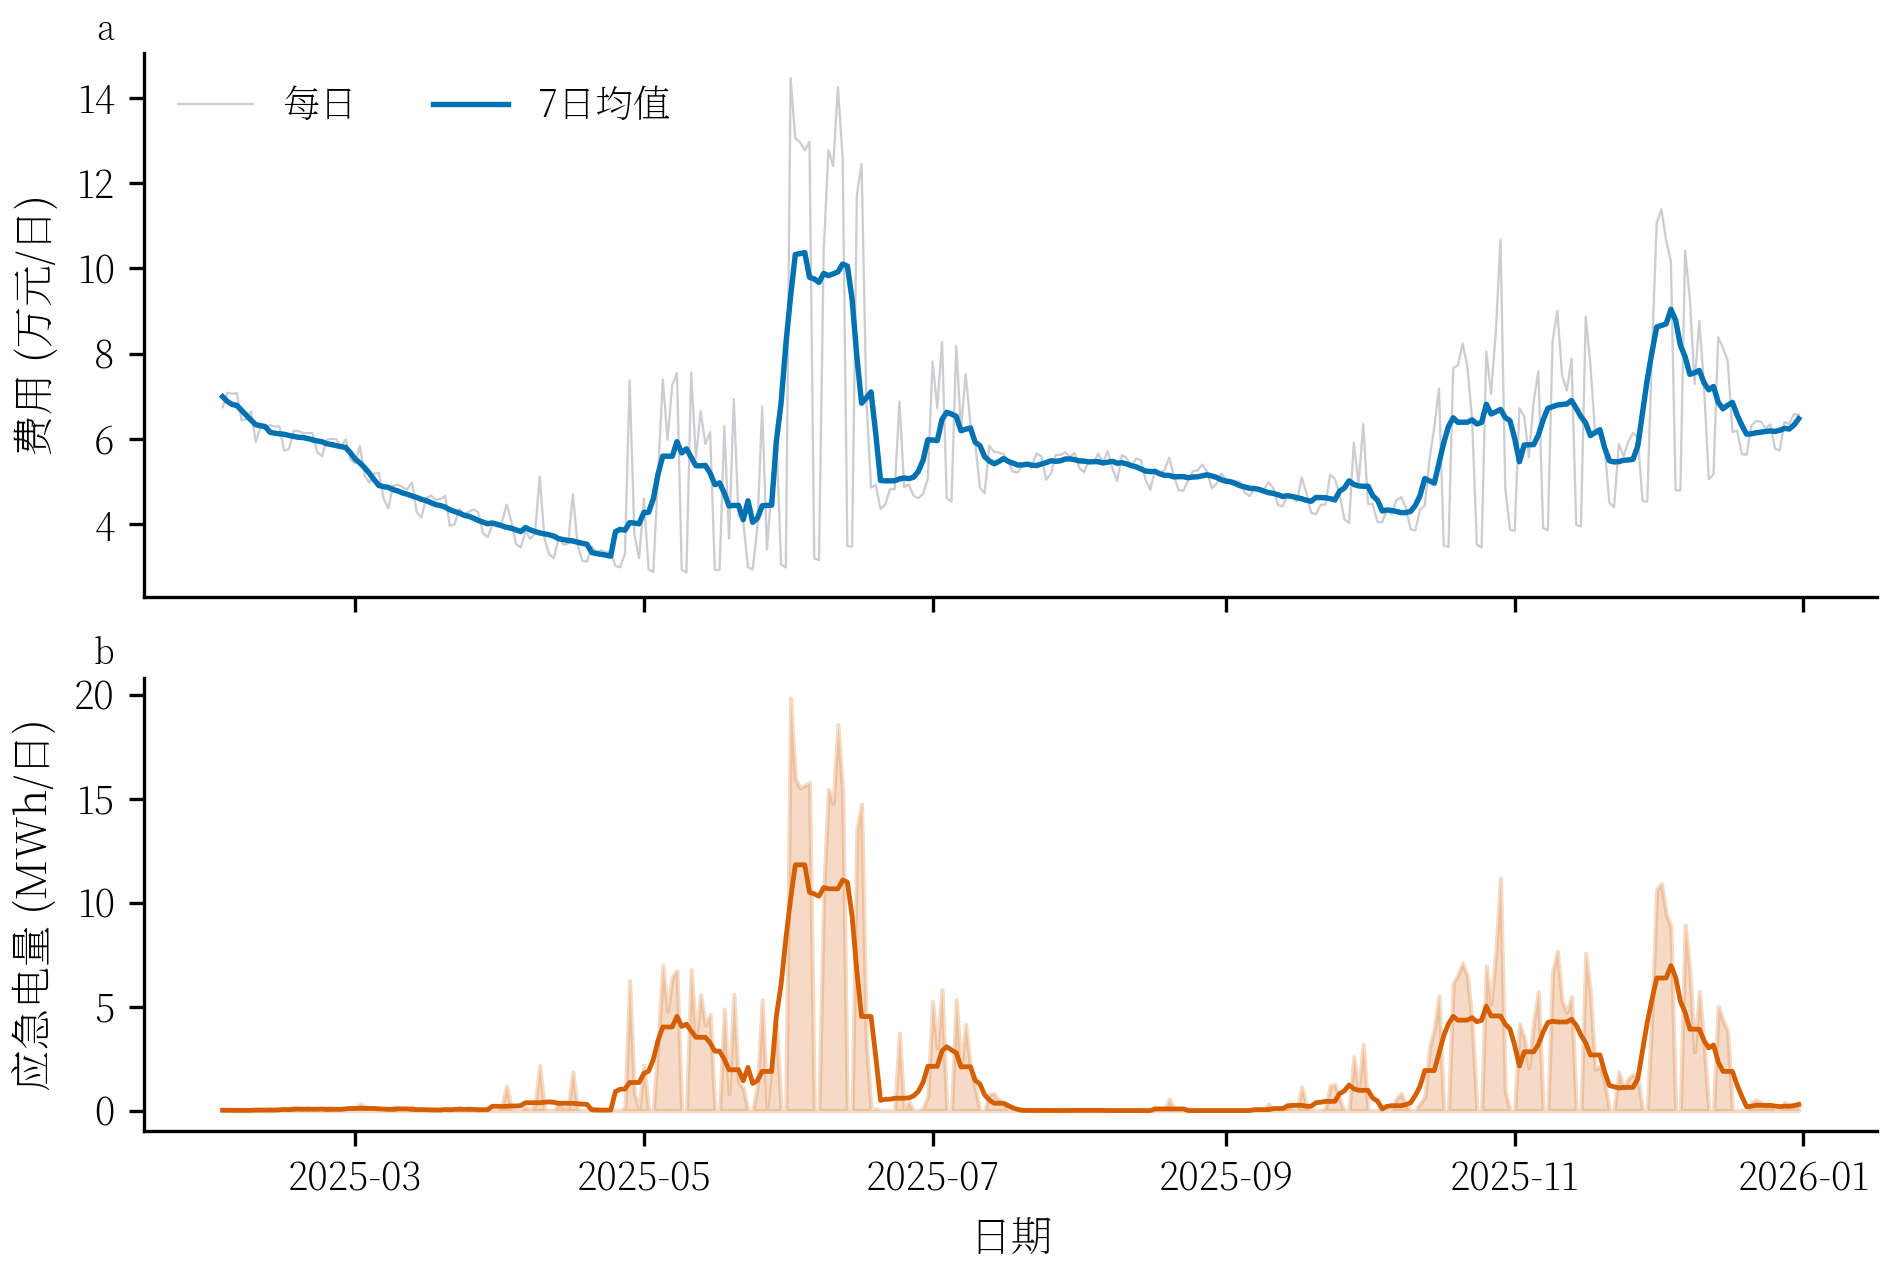
\includegraphics[width=0.98\textwidth]{figs/result_q2_annual_risk.png}
  \caption{问题二334日现金费用与应急购电量。原始日值显示尾部风险，中心均线不作为模型输入。}
  \label{fig:q2-risk}
\end{figure}

为判断保守轨迹的作用，比较点预测、典型日和无储能三类基线。表\ref{tab:q2base}显示，点预测和典型日方案都因应急购电显著增加而费用较高。无储能方案费用低于这两项，却仍高于保守轨迹主策略；它的应急量与主策略相近，但弃光更高，说明储能和合同保守度必须联合考察，不能只看应急电量。

\begin{table}[H]
\centering
\caption{问题二主策略与基线的334日结果}
\label{tab:q2base}
\begin{tabular}{lrrr}
\toprule
策略 & 现金费用/元 & 应急购电/kWh & 弃光/kWh\\
\midrule
保守分位轨迹 & 18,764,165.93 & 578,081.54 & 1,950,263.98\\
点预测 & 27,574,292.97 & 2,685,630.97 & 1,618,696.22\\
典型日 & 27,753,076.30 & 2,724,419.83 & 1,773,185.71\\
无储能 & 21,799,176.46 & 609,913.86 & 3,058,159.92\\
\bottomrule
\end{tabular}
\end{table}

\noindent 图\ref{fig:q2-baselines}进一步把合同结算与应急费用分开。主策略普通合同部分较高，是对预测尾部风险的事前支付；点预测和典型日虽然减少合同购买，却把更多缺口暴露在5倍应急价格下。无储能方案没有充放损耗，但中午光伏难以跨时段转移，其弃光约305.82万kWh，显著高于有储能主策略。由此，主策略的优势不是单纯“买得更多”或“电池越大越好”，而是合同保守度与储能转移共同改变了高价缺口的位置和规模。

\begin{figure}[H]
  \centering
  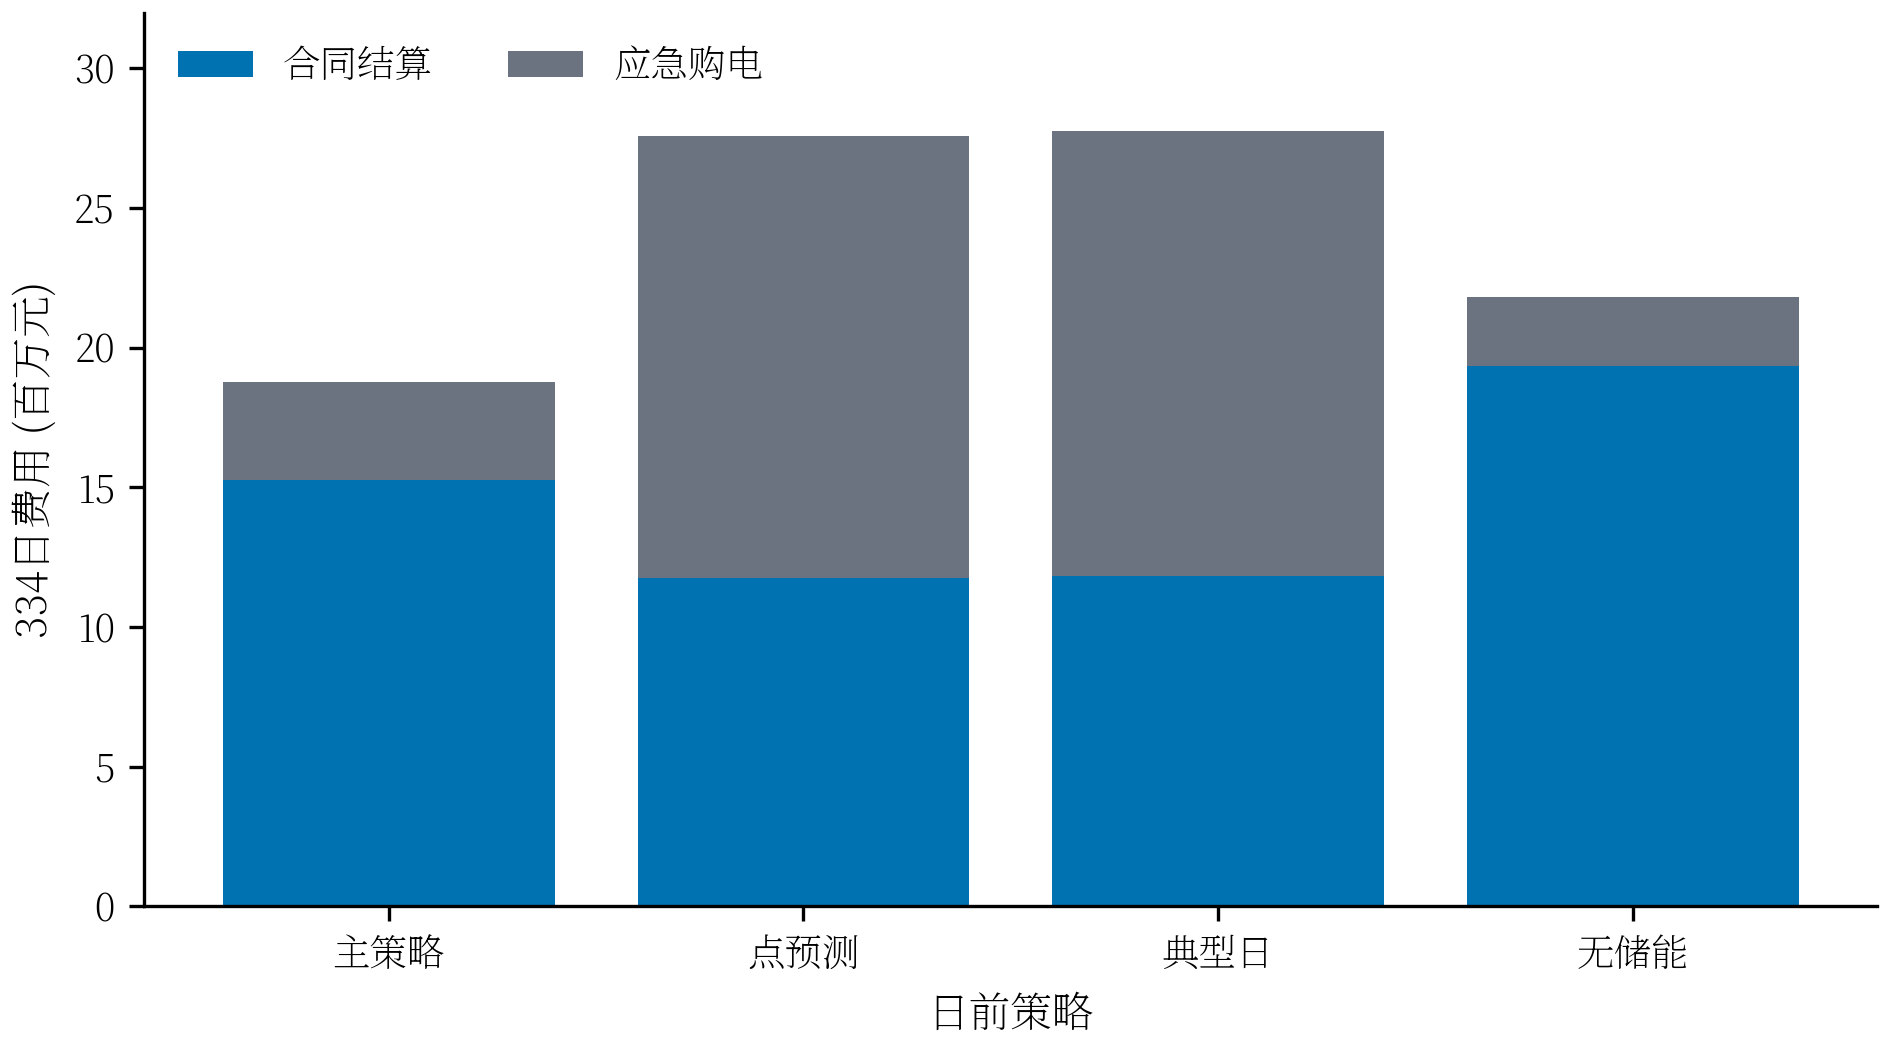
\includegraphics[width=0.96\textwidth]{figs/result_q2_baselines.png}
  \caption{问题二不同基线的合同费用与应急费用分解。柱高为334日总额，不表示抽样均值的置信区间。}
  \label{fig:q2-baselines}
\end{figure}

四个代表日的指定购电、储能和应急表分别列于附录\ref{app:tables}。代表日结果同时显示一个重要边界：策略在总体上降低风险，并不意味着每个日期都严格优于其他策略；这种日期异质性将在问题三中继续讨论。

\section{问题三：日内光伏预报与合同调整}

\subsection{官方预报的因果处理}

附件给出0、6、12、18时发布的逐小时光伏预报。对发布时刻 $h\in\{0,6,12,18\}$，先将未来整点预报裁剪为非负，再以当前时刻已经观测的光伏端点为锚，线性插值到10分钟网格。1月1日0时没有前一已观测端点，锚值取0。这样既避免光伏出现负值，也防止插值曲线在更新时刻与真实已观测前缀脱节。

令 $F_{d,h,\ell}$ 为日$d$在时刻$h$对提前 $\ell$ 小时目标的官方预报，真实值为 $V_{d,h+\ell}$。偏差样本定义为
\begin{equation}
 r_{d,h,\ell}=V_{d,h+\ell}-F_{d,h,\ell}.
 \label{eq:official-residual}
\end{equation}
在日期$d$进行修正时，只取最近60个已完成日期的同一发布时刻残差均值，不能使用当天尚未完成的残差。经非负裁剪的修正预报为
\begin{equation}
 \widehat V^{\mathrm{off}}_{d,h,\ell}
 =\max\left\{0,F_{d,h,\ell}+\frac{1}{|\mathcal R_{d,h}|}
 \sum_{k\in\mathcal R_{d,h}}r_{k,h,\ell}\right\}.
 \label{eq:bias-correction}
\end{equation}
若历史为空，则修正量为0。

图\ref{fig:q3-error}给出原始预报误差随发布时间和提前期的变化。对相同的当日剩余目标，0、6、12、18时原始MAE分别为186.7347、129.0903、35.1985和0.00036 kW，修正后分别为188.1883、130.9920、35.5854和0.00051 kW。修正降低了平均偏差的绝对值，但MAE并未改善；18时剩余目标主要处于夜间，满足真实光伏大于100 kW的MAPE有效样本数为0，故不报告MAPE数值。该结果说明“消除均值偏差”不等同于“降低绝对误差”。

\begin{figure}[H]
  \centering
  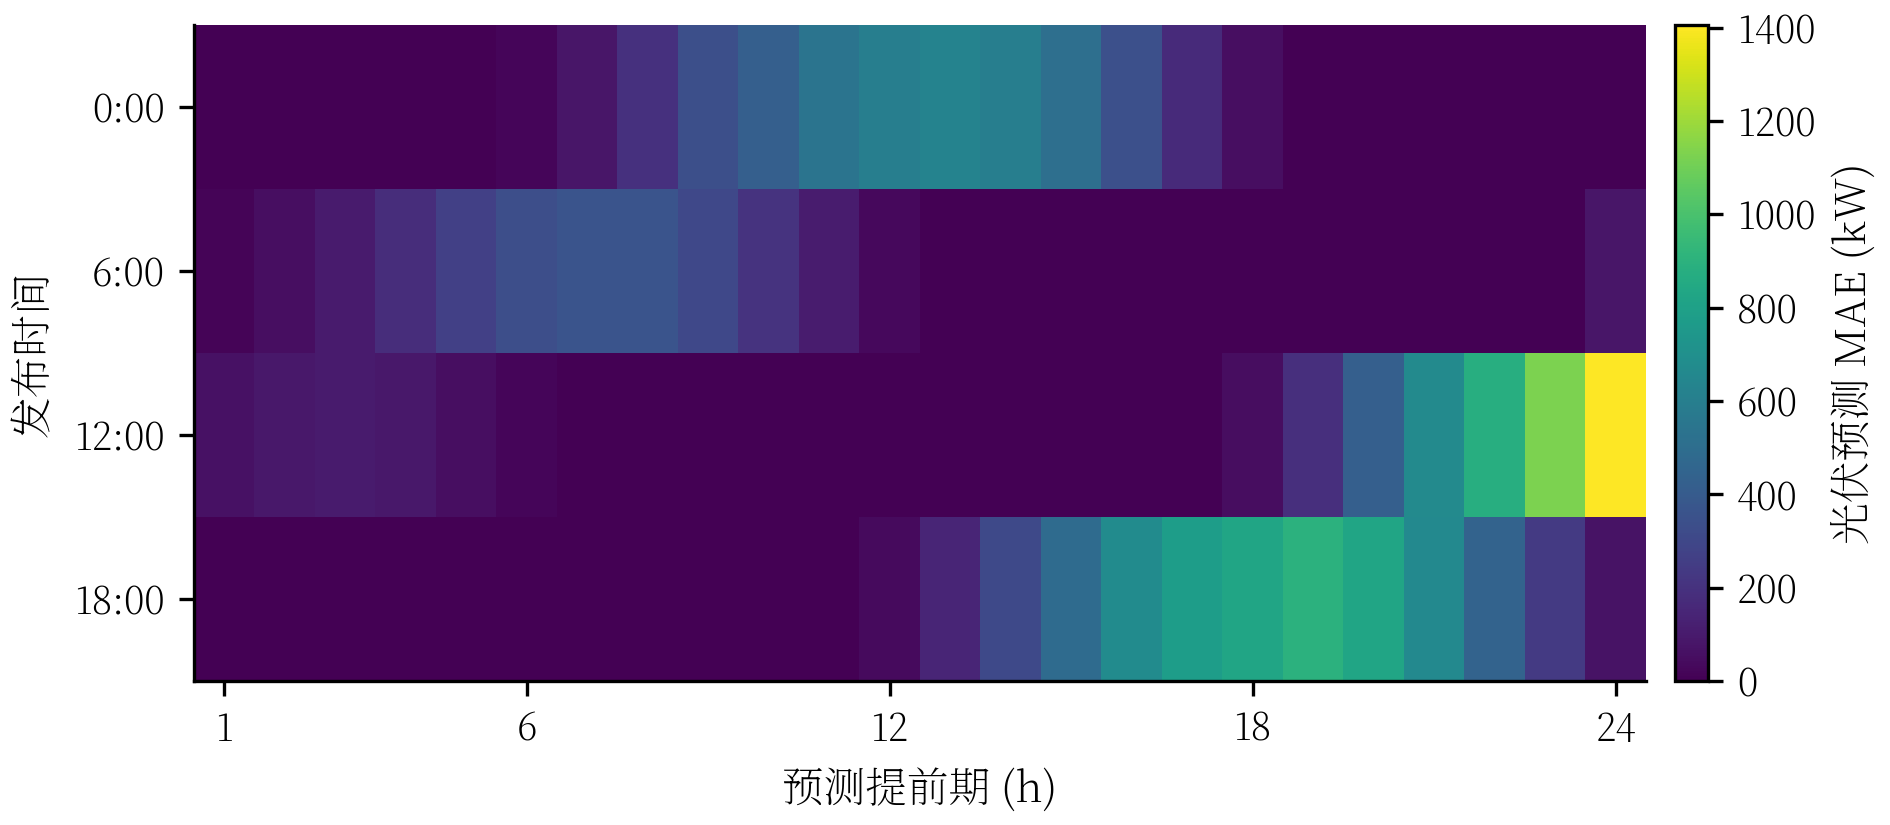
\includegraphics[width=0.98\textwidth]{figs/raw_q3_forecast_error.png}
  \caption{官方光伏预报MAE随发布时刻与提前期的变化。跨年不可得目标被排除，颜色不代表概率置信度。}
  \label{fig:q3-raw}
  \label{fig:q3-error}
\end{figure}

\subsection{滚动合同与结算模型}

0时先生成全天合同 $p_t$。每次更新到达后，对 $t\ge 6h$、$12h$ 或 $18h$ 的尚未执行时槽重新求解，已执行合同和实际能量流保持不变。规划中的负荷预测仍来自相似日模型；安全光伏轨迹用更新后的官方预报替代点预测，并继续使用过去残差形成保守余量。当天SOC从前一事件末端传递到下一事件，不因重规划而重置。

设 $q_t$ 为某时槽最后一次更新后真正执行的合同。主结算解释以0时合同 $p_t$ 为不可变基准，并按最终合同只结算一次：
\begin{equation}
 C_t=c_t\left[\min(p_t,q_t)+1.5\pos{q_t-p_t}
 +0.5\pos{p_t-q_t}\right]+5c_tu_t .
 \label{eq:settlement-primary}
\end{equation}
其中下调合同对应半价退还的净效果；多次中间修改不逐次重复收费。为检验题意解释的影响，再对同一物理执行轨迹计算
\begin{equation}
 C_t^{\mathrm{alt}}=c_t\left[p_t+1.5\pos{q_t-p_t}
 +0.5\pos{p_t-q_t}\right]+5c_tu_t .
 \label{eq:settlement-alt}
\end{equation}
式\eqref{eq:settlement-alt}把下调量作为额外费用而非退款。它只用于同策略重新计费，没有在该规则下重新优化；在允许合同闲置且无退款收益的情况下，下调动作甚至可能被不下调严格支配。因此，两种费用必须分别解释，不能混称为同一个最优问题。

以 $p_t=10$ kWh、$c_t=1$ 元/kWh且无应急购电为例，最终合同 $q_t=5,10,15$ kWh时，主结算费用分别为7.5、10和17.5元；替代结算分别为12.5、10和17.5元。该例说明两式只在下调区间不同：主式把未执行的5 kWh基准合同按半价净退款处理，替代式则在原合同上再加半价下调费用。若不先明确这一差别，同一合同轨迹会得到不同的频率建议。

滚动求解还必须保持事件间状态一致。设相邻更新时刻为 $h_j<h_{j+1}$，在 $h_j$ 只求解尚未执行的剩余段；区间 $[h_j,h_{j+1})$ 按真实值执行后，得到的SOC是下一次LP的固定初态。已执行合同、充放电和应急量均不回写。因而最终日费用可以按144个槽各自的最后有效合同相加，而不能把四次规划目标相加。

图\ref{fig:q3-update}展示6月21日合同随预报更新发生有方向的改变。图中的实际净负荷尚未扣除储能动作，因此不能把合同曲线与净负荷曲线的差直接解释为应急量或弃光量。

\begin{figure}[H]
  \centering
  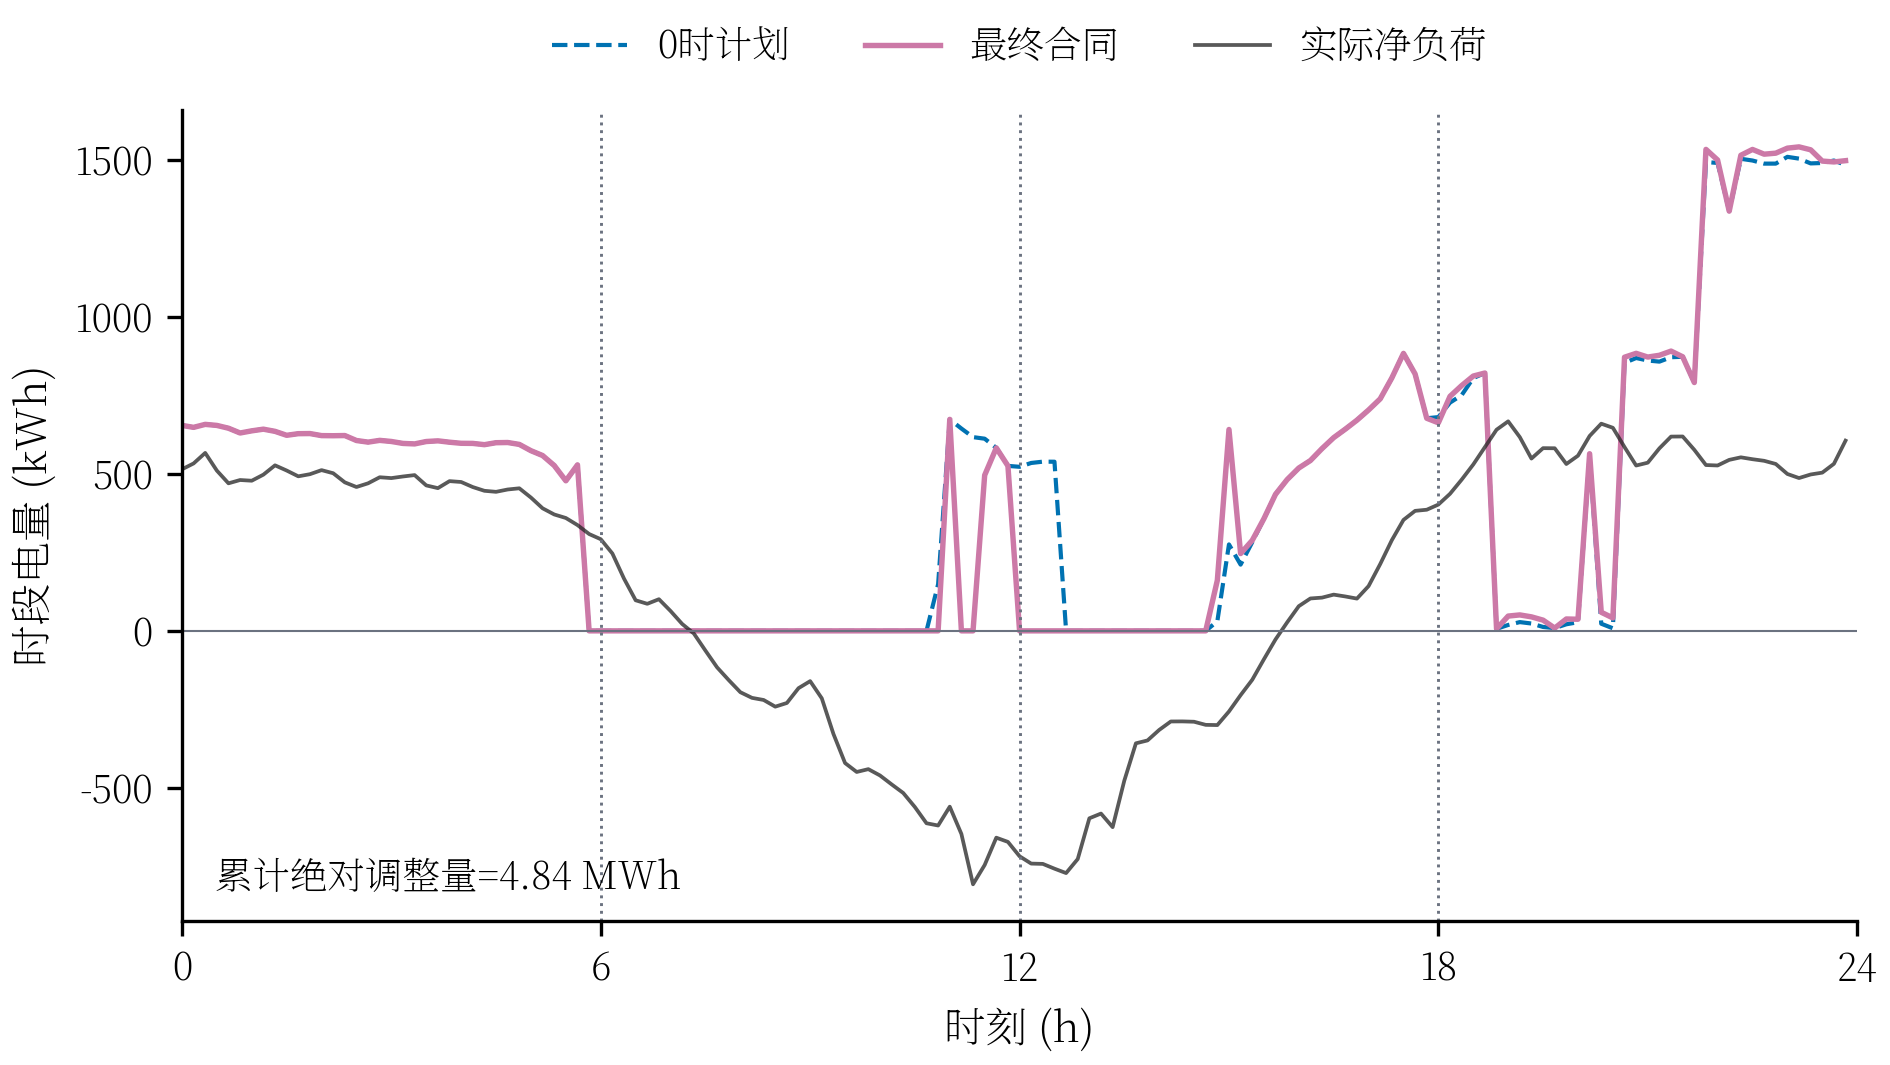
\includegraphics[width=0.97\textwidth]{figs/process_q3_contract_updates.png}
  \caption{6月21日0时初始合同与日内最终合同。竖线为6、12、18时更新事件。}
  \label{fig:q3-update}
\end{figure}

\subsection{主策略结果}

问题三334日现金费用为 $16279696.6905$ 元，应急购电量为 $115458.1457\,\mathrm{kWh}$，闲置合同为 $3093394.8432\,\mathrm{kWh}$，弃光为 $1841583.5122\,\mathrm{kWh}$，年末SOC为 $10649.4342\,\mathrm{kWh}$。相对问题二，现金费用减少 $2484469.2430$ 元，应急购电减少约80.03\%。但这项差异同时改变了光伏信息来源和合同更新规则，并非“只增加更新次数”的纯频率效应。

四个代表日中，3月20日、6月21日和9月23日费用下降，而12月21日费用由 $63120.3057$ 元上升为 $65731.5948$ 元，应急购电也从 $382.2268$ 增至 $979.7444\,\mathrm{kWh}$。因此，年度改善不能被写成逐日占优。详细代表日购电、储能与应急结果见附录\ref{app:tables}。

\subsection{相同0时信息下的更新频率分析}

为尽量分离“0时信息不同”的影响，固定0时采用问题三的同一官方信息，比较只在0时、0/12时、0/6/12/18时和每2小时更新四组方案。2小时情形并非附件提供的新官方预报：在非官方发布时刻，模型沿用最近一次已发布预报，并以当天已经实现的最多18个10分钟槽偏差构造3小时指数衰减的合成短临更新；该更新只调整安全光伏，同时保持安全负荷轨迹，不重新标定场景概率。

\noindent 四组费用及两种结算的对照列于表\ref{tab:q3freq}。负的“相对6小时节约”表示候选方案更贵，而不是负费用。

\begin{table}[H]
\centering
\caption{固定电价下相同0时信息的更新集合比较}
\label{tab:q3freq}
\resizebox{\textwidth}{!}{%
\begin{tabular}{lrrr}
\toprule
更新集合 & 主结算费用/元 & 相对6小时节约/元 & 替代结算相对6小时节约/元\\
\midrule
仅0时 & 17,613,329.64 & $-1,333,632.95$ & $-537,280.34$\\
0、12时 & 17,143,902.65 & $-864,205.96$ & $-659,112.90$\\
每6小时 & 16,279,696.69 & 0 & 0\\
每2小时合成更新 & 15,571,353.39 & 708,343.30 & 127,065.26\\
\bottomrule
\end{tabular}}
\end{table}

2小时方案在主结算下相对6小时方案节约4.3511\%，全年增加2672次更新。若每次额外更新的综合通信、计算和运维成本记为$k$，则其净收益为
\begin{equation}
 B_{2h}=708343.3002-2672k.
 \label{eq:breakeven-fixed}
\end{equation}
故盈亏平衡阈值为 $k^*=265.0985$ 元/次。四个代表日在主结算口径下均不劣，但替代结算下总节约仅约12.71万元，且仅0时与12小时方案的排序会反转。图\ref{fig:q3-frequency}直观显示结算解释对更新价值的影响，因此合理建议是“在主结算成立且每次增量成本低于阈值时采用2小时合成更新”，而不是无条件追求最高更新频率。

\begin{figure}[H]
  \centering
  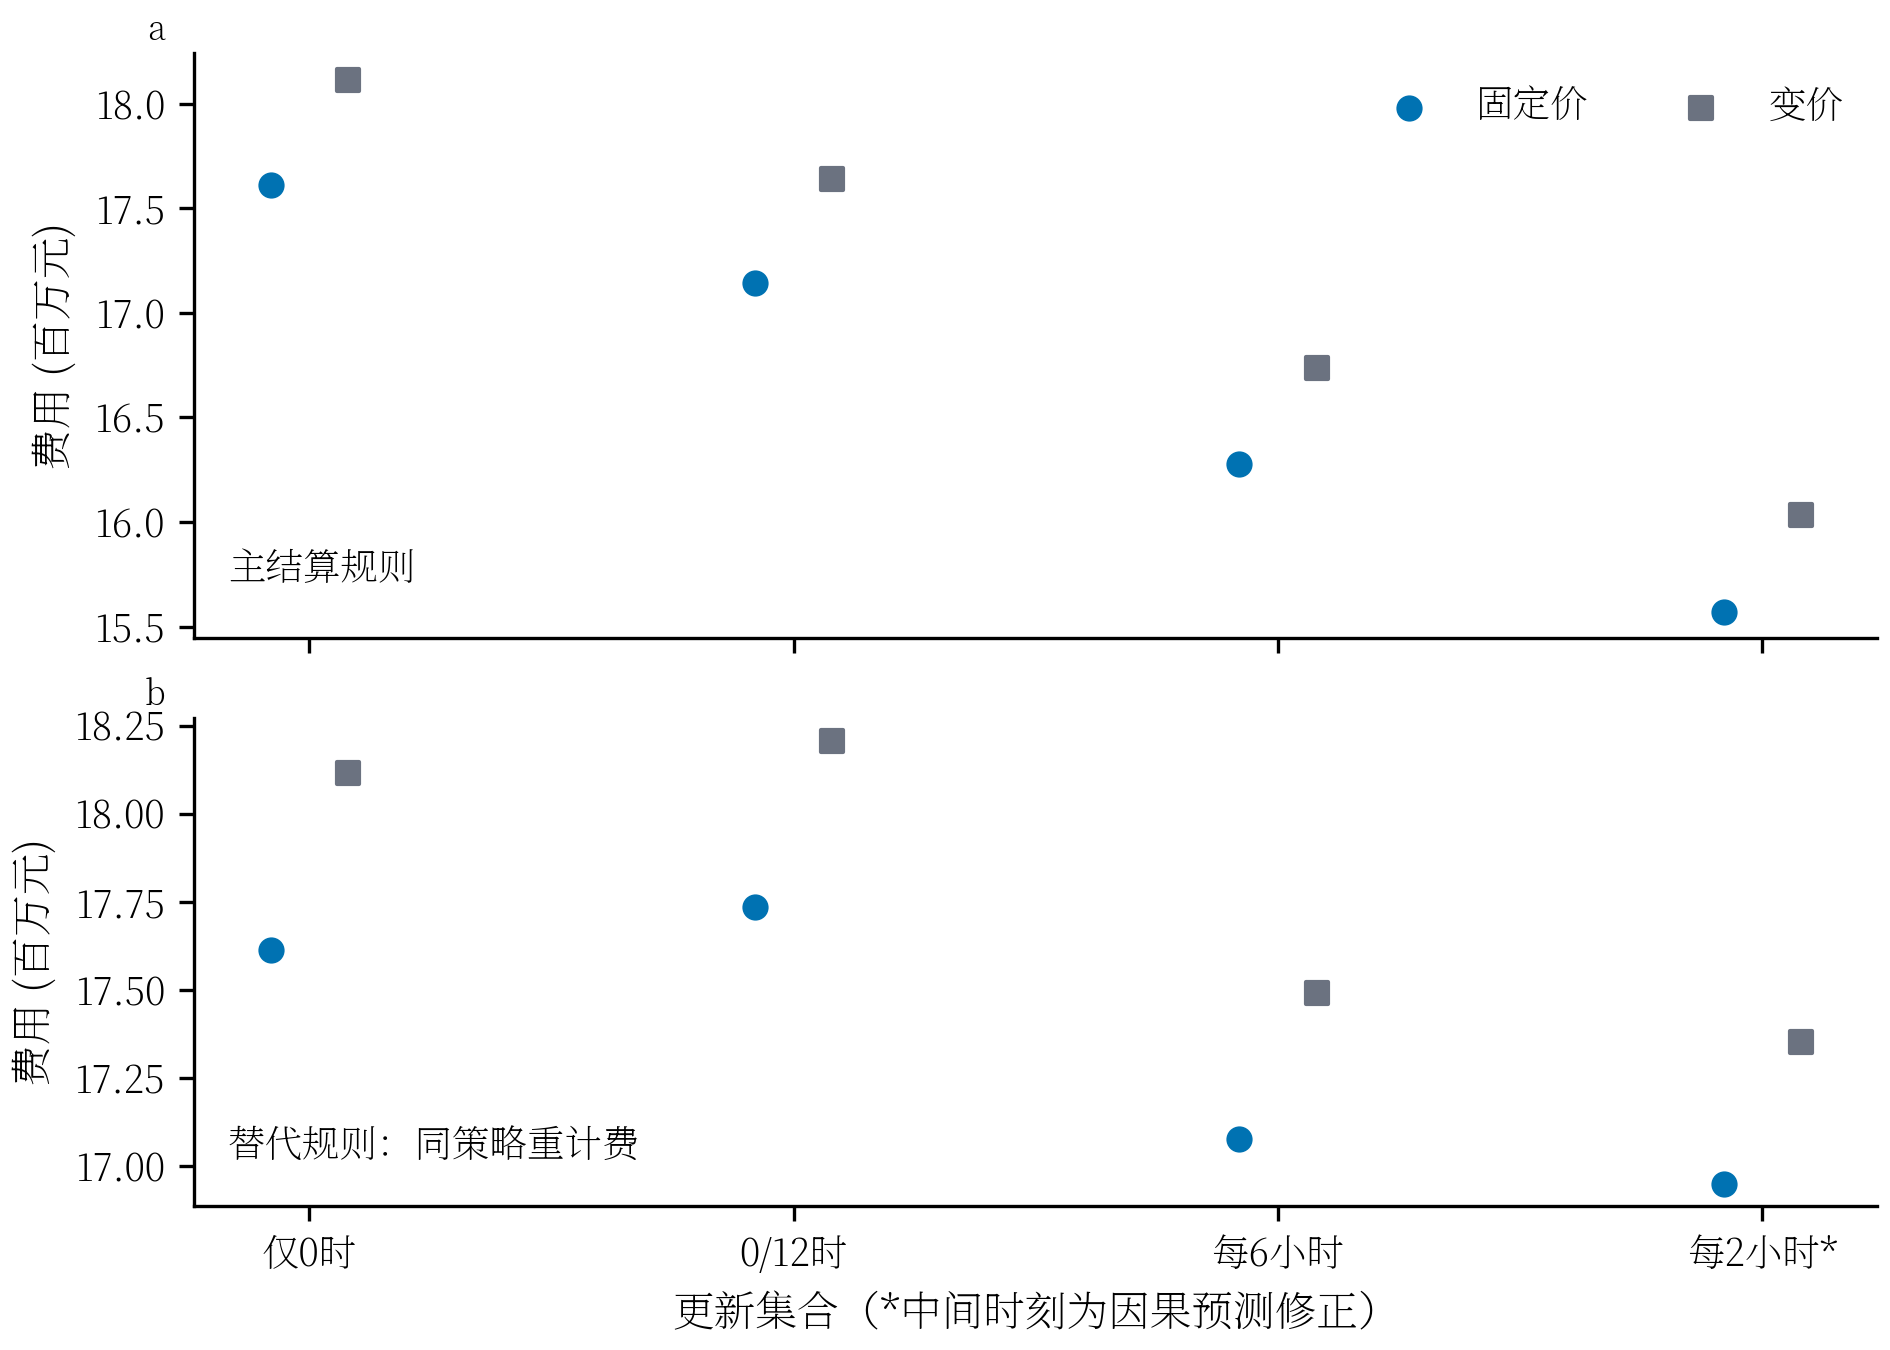
\includegraphics[width=0.96\textwidth]{figs/result_q3_update_frequency.png}
  \caption{固定与变动电价下不同更新集合的总费用，分别按主结算和替代结算重计。2小时方案使用因果合成更新。}
  \label{fig:q3-frequency}
\end{figure}

\section{问题四：变动电价下的滚动调度}

\subsection{未来价格的因果预测}

问题四的实际电价随日期和时槽变化。若在规划时直接读取当天未来真实价格，会产生明显的未来信息泄漏。本文对日期$d$、槽$t$的0时价格预测取过去30日同槽价格的中位数：
\begin{equation}
 \widehat c_{d,0,t}=\operatorname{median}\left\{c_{k,t}:\max(0,d-30)\le k<d\right\}.
 \label{eq:price-dayahead}
\end{equation}
首日没有历史时使用附件典型价格。日内时刻$h$重新规划时，计算当天已经实现的最近至多18槽价格偏差中位数 $b_{d,h}$，并按3小时尺度向未来衰减：
\begin{equation}
 \widehat c_{d,h,t}=\max\left\{10^{-4},\widehat c_{d,0,t}
 +b_{d,h}\exp\left[-\frac{t-t_h}{18}\right]\right\},\quad t\ge t_h .
 \label{eq:price-intraday}
\end{equation}
其中 $t_h=6h$。规划目标使用 $\widehat c$，真实 $c$ 仅用于合同和应急费用结算。图\ref{fig:q4-price}显示各月价格分布具有离散性和尾部，故单一月均价不足以描述调度机会；箱线图中的离群点均被保留。

中位数而非均值用于0时价格预测，是因为月内价格分布包含尾部，少数尖峰会明显拉动均值。该选择并不意味着忽略尖峰：安全供能仍由负荷和光伏分位轨迹控制，而价格中位数只决定有限电池能量在剩余时槽间的相对配置。当日偏差项使整体价格水平随已实现数据上移或下移，指数衰减则避免把刚刚发生的局部异常永久外推到全天。

在实际执行时，储能动作与真实价格的相关性只能作为事后描述，不能反向证明控制器预知价格。规划时可利用的是 $\widehat c_{d,h,t}$；真实 $c_{d,t}$ 在槽结束时进入结算。若实际高价尖峰未被历史中位数和已实现偏差预见，策略可能保留不足的SOC，这正是个别代表日有调账方案费用反而上升的可能机制之一。

\begin{figure}[H]
  \centering
  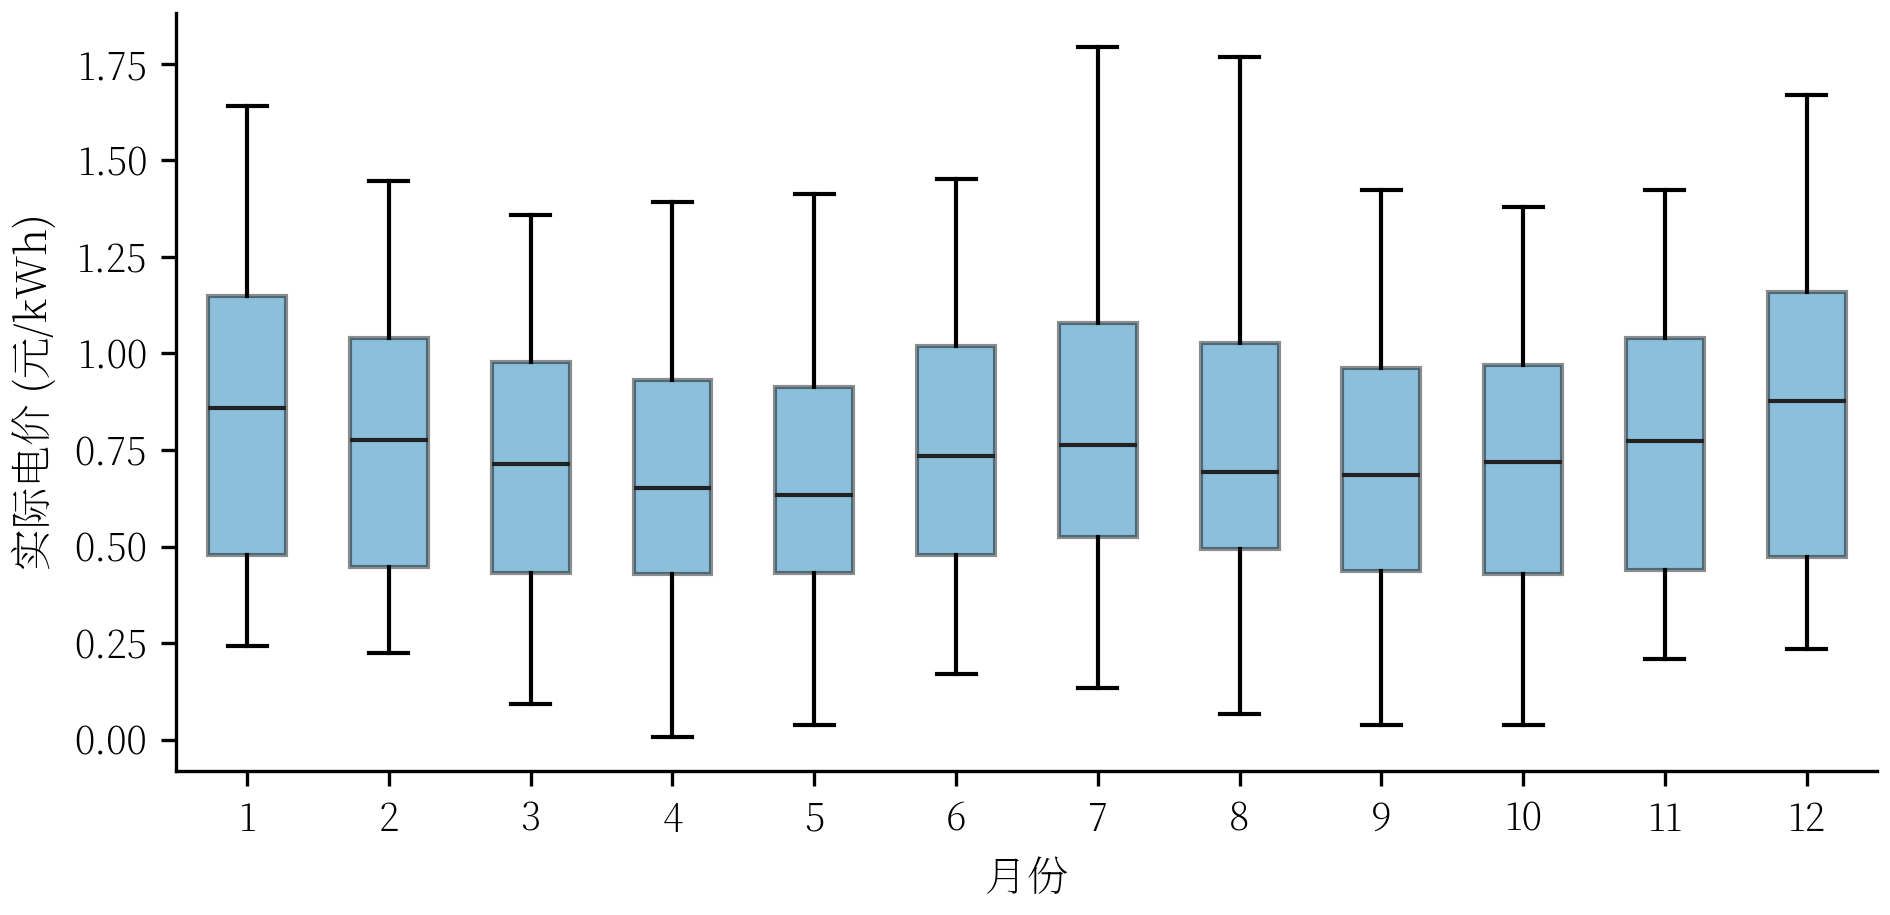
\includegraphics[width=0.98\textwidth]{figs/raw_q4_price_variability.png}
  \caption{2025年各月10分钟电价分布。箱体为四分位区间，须线为1.5倍四分位距，离群点未删除。}
  \label{fig:q4-price}
\end{figure}

\subsection{两种策略及结果}

问题四的无调账方案沿用问题二的相似日与分位轨迹，只把固定价目标替换为式\eqref{eq:price-dayahead}的预测价格；有调账方案沿用问题三的0、6、12、18时更新机制，并在每次滚动求解时使用式\eqref{eq:price-intraday}。两者执行层均只读取当前真实量，储能跨日连续。

表\ref{tab:q4main}给出正式统计结果。有调账方案比无调账方案节约 $2519380.1148$ 元，应急购电减少 $459960.1389\,\mathrm{kWh}$。若把问题二和问题三也纳入同一图，固定价与变价都呈现“有调账总体费用更低”的结果，见图\ref{fig:q4-result}。但是，固定价的$q2\to q3$和变价的$q4\_2\to q4\_3$都同时改变了信息与更新规则，不能当作单因素频率效应。

\begin{table}[H]
\centering
\caption{问题四两个方案的334日结果}
\label{tab:q4main}
\begin{tabular}{lrrrr}
\toprule
方案 & 现金费用/元 & 应急/kWh & 闲置合同/kWh & 弃光/kWh\\
\midrule
无调账 & 19,254,498.44 & 575,898.35 & 4,100,533.58 & 1,969,275.57\\
有调账 & 16,735,118.32 & 115,938.21 & 3,085,161.95 & 1,848,622.33\\
\bottomrule
\end{tabular}
\end{table}

\begin{figure}[H]
  \centering
  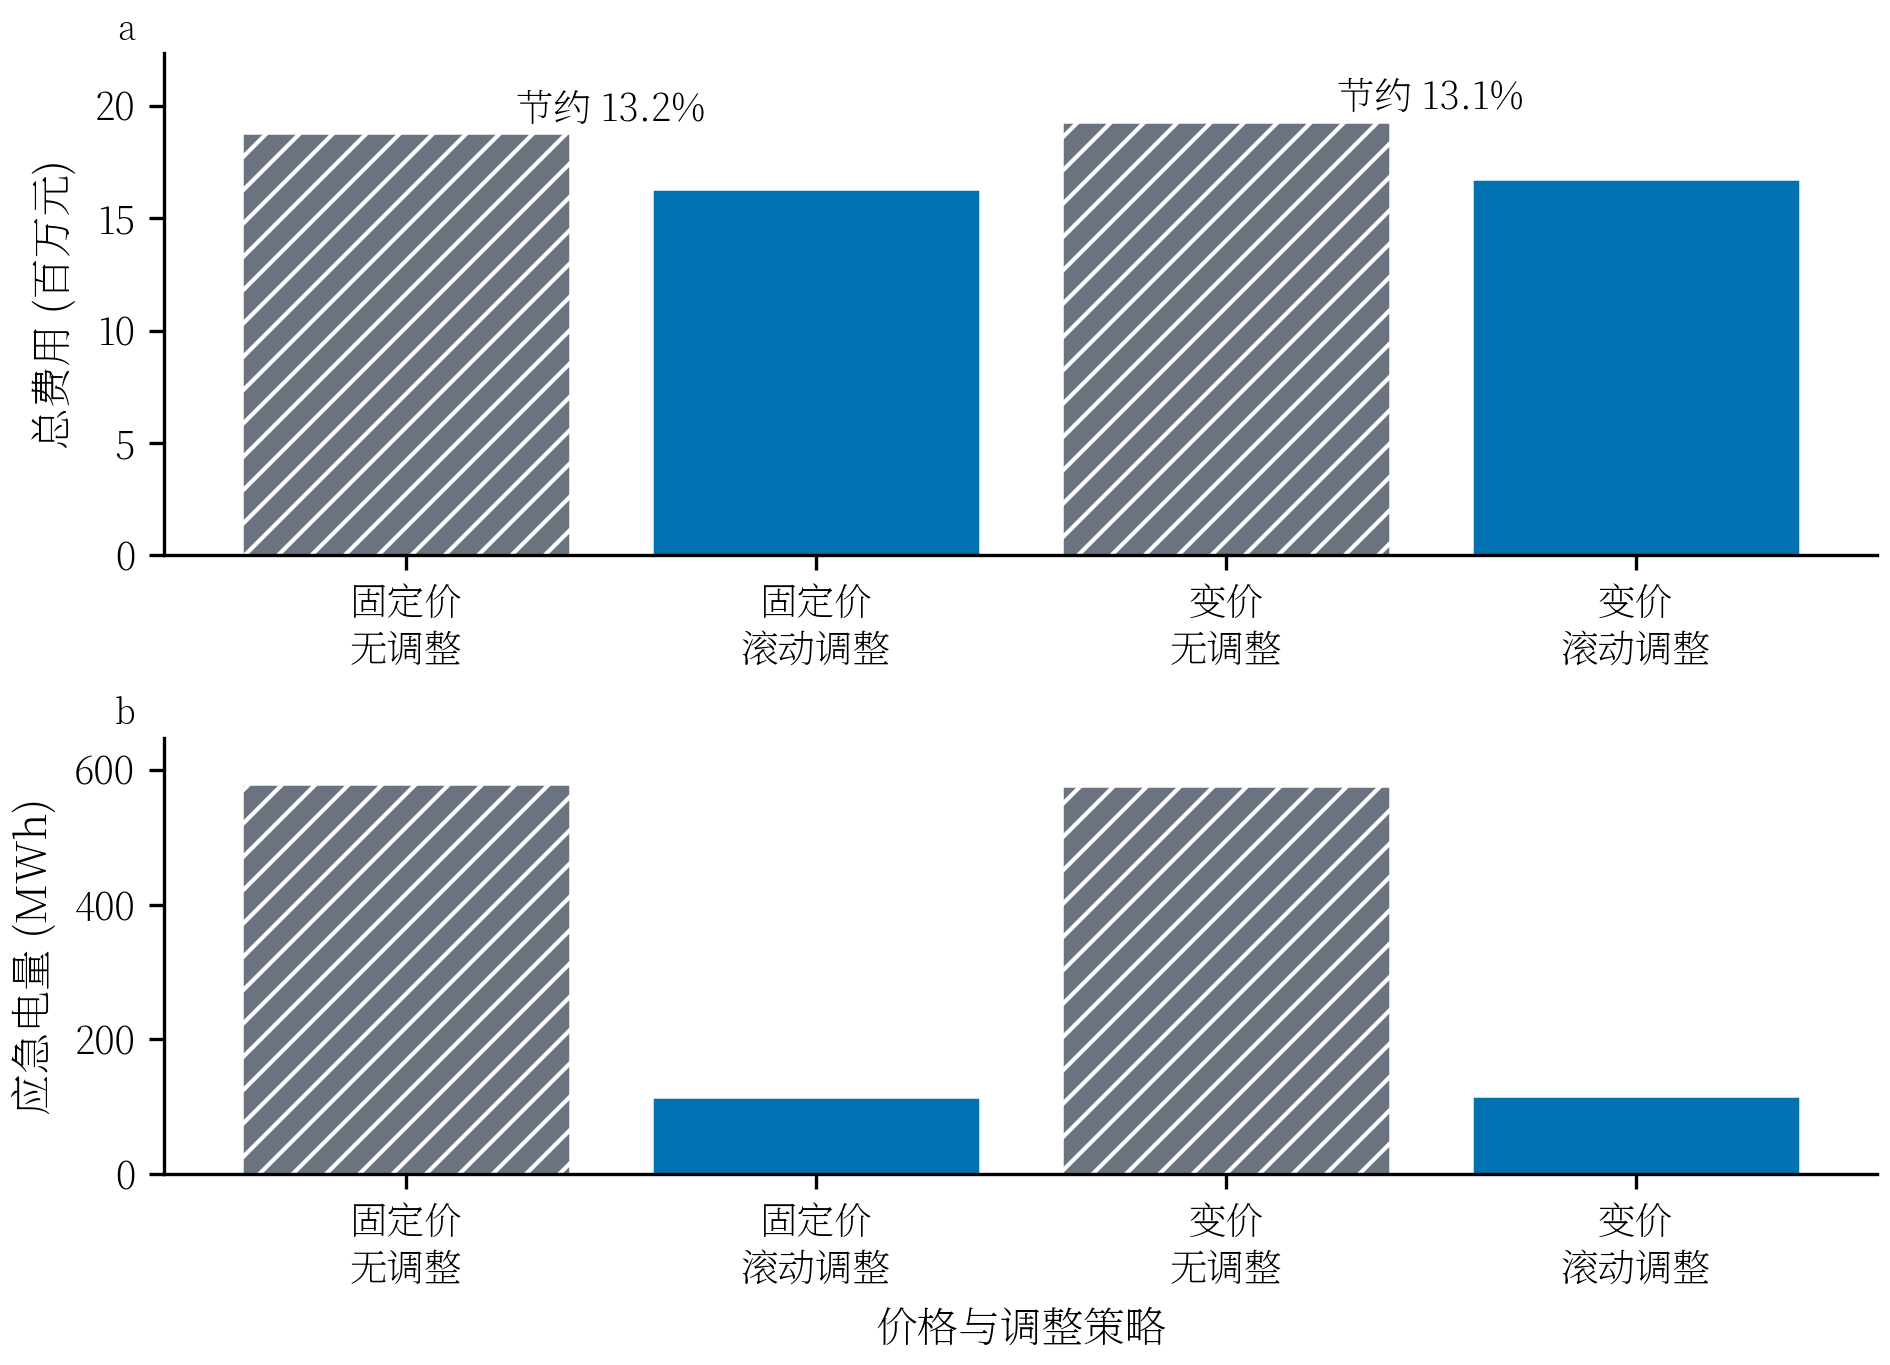
\includegraphics[width=0.96\textwidth]{figs/result_q4_strategy_comparison.png}
  \caption{固定价与变动电价下四个主策略的334日费用和应急购电量。}
  \label{fig:q4-result}
\end{figure}

代表日同样并非全部改善：12月21日无调账方案费用为 $74025.4512$ 元，有调账方案反而为 $77842.3118$ 元。其应急电量由 $382.2268$ 变为 $978.6827\,\mathrm{kWh}$。这说明滚动预测在总体上更有效，却可能在个别日期因预报误差、储能边界和价格预测偏差叠加而失利。两方案的完整代表日指定表见附录\ref{app:tables}和配套工作簿。

\subsection{变价条件下的更新频率建议}

在相同0时信息下，变价2小时合成更新方案费用为 $16033486.6253$ 元，6小时方案为 $16735118.3246$ 元，前者节约 $701631.6992$ 元，即4.1926\%。两方案相差2672次更新，故净收益为
\begin{equation}
 B^{\mathrm{var}}_{2h}=701631.6992-2672k,
 \label{eq:breakeven-variable}
\end{equation}
盈亏平衡阈值为 $262.5867$ 元/次。若采用替代结算式\eqref{eq:settlement-alt}对同一策略重计费，节约额缩小为 $139845.6748$ 元，不能把主结算阈值直接移用于该口径。

因此，问题四的建议为：在题设主结算解释成立、能够可靠取得最新官方预报和已观测前缀，且单次增量更新成本低于约262.59元时，可采用2小时合成更新；否则6小时官方发布节奏具有更稳健的实施性。2小时结果仅表示本题数据上的因果短临更新价值，不代表系统获得了额外官方预报产品。

\section{模型检验、敏感性与稳健性分析}

\subsection{物理可行性与因果性检验}

对问题一及四个年度主策略逐槽检查式\eqref{eq:balance}、式\eqref{eq:soc}、SOC边界、充放电功率、非负性、同时充放和跨日连续性。问题一最大母线平衡残差为 $9.10\times10^{-13}\,\mathrm{kWh}$；四个主策略正式统计期的最大平衡残差不超过 $3.70\times10^{-13}\,\mathrm{kWh}$，独立逐槽重算的最大SOC递推残差约为 $4.55\times10^{-12}\,\mathrm{kWh}$。这些量接近浮点运算精度，表明结果满足模型物理方程。

因果性检验在第0、1和364日的0、2、\ldots、22时，对未来负荷、光伏、价格和未发布预报分别作36组扰动。当前预测、价格估计和当前LP计划的最大差均为0；已执行前缀和SOC边界也不受未来扰动影响。这验证了实现遵守信息集 $\mathcal F_{d,h}$。该检验说明“没有使用被扰动的未来数据”，但不是对所有可能代码路径的形式化证明。

\subsection{54组实验设计}

实验共54组，其中16组为固定价/变价的安全轨迹、点预测、典型日、无储能，以及0/12/6/2小时更新基线；另有38组单因素实验。单因素范围包括：
\begin{itemize}
  \item 保守分位参数 $\alpha=0.70,0.75,0.80,0.85,0.90,0.95$；
  \item 残差聚类上限5、9、12、16，残差历史30、60、90日；
  \item 储能容量和功率分别为主值的0.8、1.0、1.2倍；
  \item 往返效率从0.81提高到0.90，即单向效率改为 $\sqrt{0.9}$；
  \item 应急电价倍率3、4、5、6、8。
\end{itemize}
容量改变时，SOC下限、上限和初态仍分别为容量的10\%、90\%和50\%，而功率与效率保持不变；功率实验则不改变容量。应急倍率实验固定物理策略和 $\alpha=0.8$，只重新计算费用暴露，因此不能称为各倍率下重新寻优的最优策略。

\subsection{保守参数与设备参数}

图\ref{fig:q4-alpha}展示 $\alpha$ 对费用和应急量的权衡。固定价问题二中，$\alpha=0.95$ 的样本内费用低于主设定0.8；变价有调账方案中，0.8是测试点中的最低费用。由于主参数在查看本年度结果前固定，本文不据此把0.95或0.8宣称为普适最优参数。样本内曲线的主要价值在于说明保守度改变会同时影响合同过购、应急缺口和弃光，而不是提供无偏超参数选择。

\begin{figure}[H]
  \centering
  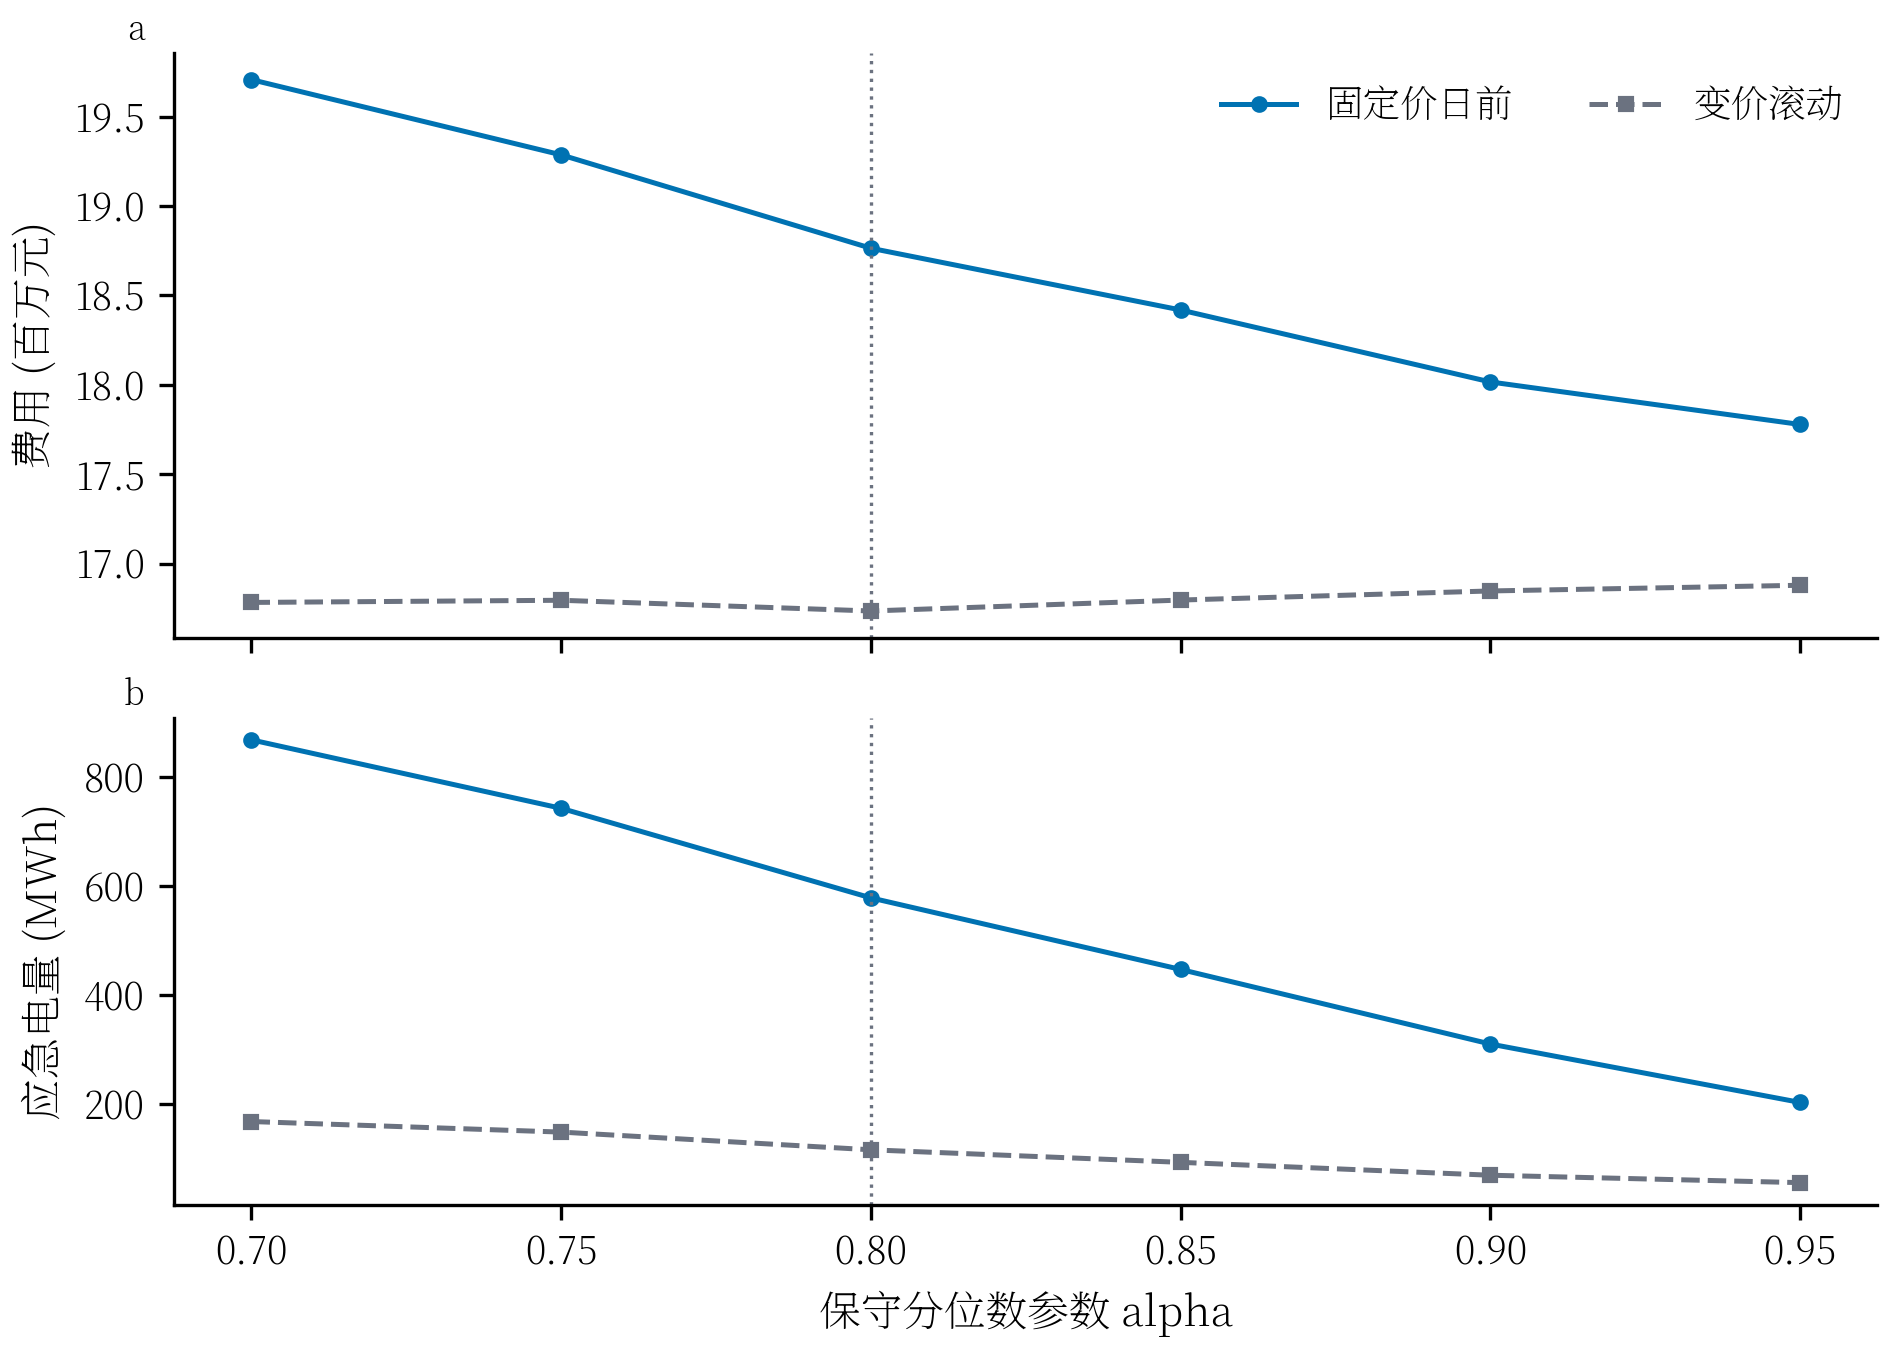
\includegraphics[width=0.96\textwidth]{figs/result_q4_alpha_sensitivity.png}
  \caption{问题二与问题四有调账策略对保守分位参数的单因素敏感性。主方案 $\alpha=0.8$ 为事前固定值。}
  \label{fig:q4-alpha}
\end{figure}

历史窗口30日时，问题二和问题四有调账方案费用分别约为1698.74万元和1629.52万元；90日窗口更高。这反映2025年样本中的近期结构更有用，但不证明短历史在其他年份总是更好。容量增加20\%后，两方案费用分别约为1821.87万元和1600.59万元；容量减少20\%并不必然按比例增加费用，因为合同风险、弃光和终端SOC共同变化。

表\ref{tab:sensitivity-selected}列出若干有代表性的单因素结果。历史窗口30日对两个方案都较有利，说明2025年数据存在较强的近期性；提高往返效率则稳定降低费用。容量增加对问题四有调账方案的收益大于对问题二，原因是变价环境下额外可用能量同时具有峰谷转移和风险缓冲价值。所有比较都只改变表中一个因素，其余参数保持主设定。

\begin{table}[H]
\centering
\caption{部分单因素实验的334日现金费用（万元）}
\label{tab:sensitivity-selected}
\begin{tabular}{lrr}
\toprule
实验设置 & 问题二无调账 & 问题四有调账\\
\midrule
主设定 & 1876.42 & 1673.51\\
残差历史30日 & 1698.74 & 1629.52\\
储能容量增加20\% & 1821.87 & 1600.59\\
储能功率降至80\% & -- & 1669.53\\
往返效率提高到90\% & 1832.77 & 1620.57\\
\bottomrule
\end{tabular}
\end{table}

问题四有调账方案将功率降至主值的80\%时，样本内费用约为1669.53万元，略低于主方案1673.51万元。这一非单调性并不违反物理规律：控制器采用保守轨迹规划和真实值下的贪心执行，并非在完全信息下对全年重新全局优化；更大的设备可行域不会自动保证启发式滚动策略产生更低的实际结算费用。往返效率提高到90\%后，费用下降到约1620.57万元，符合损耗降低的方向性预期。

实验还揭示了初态与年末状态的关系。所有容量实验都从容量的50\%起步，SOC上下界同步保持10\%和90\%；这保证比较不是由绝对初态不一致造成。然而，正式费用从2月开始统计，1月调度已经把不同容量系统推进到各自状态，因此不能简单断言初始SOC影响在一个月后完全消失。本文只报告统一启动规则下的可比结果，不对无限期稳态作额外假设。

\subsection{结算与时间口径敏感性}

同一策略在主结算和替代结算下费用差异明显。问题三主策略由1627.97万元增至1707.60万元，问题四有调账策略由1673.51万元增至1749.07万元。更重要的是，2小时相对6小时的收益在替代口径下明显收缩。因此，更新频率结论必须与式\eqref{eq:settlement-primary}绑定，不能只给一个脱离合同条款的百分比。

固定价方案还出现排序反转：主结算下12小时方案费用低于仅0时方案，而替代重计费下仅0时方案约1761.33万元，反而低于12小时方案约1773.52万元。其原因不是物理供能突然变化，而是替代规则对合同下调额外收费。该现象说明，调账价值必须同时报告物理效果和条款效果；仅凭“应急减少”不足以得出经济最优结论。

时间口径实验把典型日全部槽循环平移10分钟。购电总量仅有约 $2.38\times10^{-9}\,\mathrm{kWh}$ 的浮点差，而费用下降约0.10元。结果表明年度策略量级不依赖这一微小映射，但题目指定时段数值和逐槽费用仍需要统一定义，本文采用区间终点解释。

\subsection{计算规模与结果可追溯性}

每天的规划域最多为144槽，随着日内时间推进逐步缩短。每槽包含合同、闲置合同、光伏利用、充电、放电、应急与SOC等连续变量，约束数量随剩余槽数线性增长；所有目标和约束均为线性形式，可由通用线性规划器稳定求解。残差聚类的数据矩阵最多含60个历史日期、每行288维，且簇数不超过9，因此其规模远小于把全年每个10分钟误差都展开成场景树的做法。该结构使365日连续模拟和54组实验在普通计算机上可完成，同时保留逐槽检查的可能。

为了使结果可追溯，每个策略同时保留三层输出：第一层是逐槽合同、能量流和SOC，用于检查式\eqref{eq:balance}、式\eqref{eq:soc}及指定时段；第二层是每日合同量、现金费用、应急量、闲置合同和弃光，用于代表日与时间序列分析；第三层是334日总量及实验参数，用于跨策略比较。论文中的所有汇总均从前一层按日期和时槽聚合，而不是在正文中手工修改。题目指定的五份工作簿与同一逐槽结果共用数据源，所以论文数值、代表日表和Excel输出保持同一口径。

随机性只出现在残差聚类的初始中心，随机种子固定为2026，并使用10次初始化选择较小簇内平方和的结果。经验分位数、相似日权重、价格中位数、LP和真实执行均为确定性步骤。固定种子并不说明模型没有统计不确定性，它只确保相同输入和软件环境下不会因聚类初始化改变合同轨迹。真正的外部不确定性仍来自未来负荷、光伏和价格，已通过滚动历史、分位参数与应急购电显式暴露。

结果解释遵循“数值可行、因果可用、外部有效性待检验”的层次。逐槽残差接近机器精度证明计算结果满足本文方程；未来扰动不影响当前决策证明实现遵守给定信息边界；54组实验说明主要参数变化下结论如何移动。但这些证据不能自动证明另一年份、另一微网或另一合同条款下仍有同样节约率。工程迁移时应先复现输入映射和结算，再用滚动样本外数据重新校准历史窗口与保守度。

\subsection{模型优点与局限}

本文方法具有四点优点：第一，信息集明确，预测与执行均可通过未来扰动验证；第二，物理层完全线性，所有10分钟结果可逐槽复核；第三，联合残差在压缩前同时包含负荷和光伏误差，较单独安全系数更贴近净负荷风险；第四，两种结算、多个更新集合和设备参数均有真实重算或同策略重计费结果。

局限也十分明确。其一，边际分位压缩会丢失跨时段联合概率，不能提供机会约束保证。其二，相似日和历史中位数属于低参数预测，可能无法捕捉节假日、极端天气或结构突变。其三，真实执行采用优先级规则而非全年完美信息优化，设备参数的实际费用可能非单调。其四，储能老化、备用、配网潮流和需求响应不在题设数据中，本文没有虚构这些成本；若用于工程实施，应加入退化成本、网络约束和滚动终端集合。其五，2小时方案是由已发布预报与观测构成的合成短临结果，不能替代对真实高频预报服务的独立评估。

\section{结论与实施建议}

本文用统一的10分钟规划与执行方程连接四个问题，并将“当时可得信息”作为滚动决策的硬边界。核心方法是“合同层滚动线性规划 + 因果贪心反馈”：规划层基于预测轨迹确定合同与目标SOC，执行层在真实量逐槽到达后完成光伏消纳、充放电和应急记账。

第一，典型日连续LP得到购电 $59482.6982\,\mathrm{kWh}$、费用 $35126.9489$ 元。在6000 kWh循环SOC约束下，储能完成低价充电与高价放电，给出了后续全年模型的物理和量纲基线。

第二，固定价格且不能日内调账时，最近60个已完成日期的原始联合残差被用于提取“联合残差特征提取后的边际分位安全轨迹”。正式模式不聚类、$\alpha=0.8$ 事前冻结，所得334日现金费用为1844.64万元，应急购电49.95万kWh。与固定参数的聚类压缩对照相比，未聚类模式在问题二和问题三上均同时满足覆盖率不降低、Pinball损失不增加、费用不增加和应急量不增加，因而被选为正式主线；这项模型仍是确定性分位轨迹LP，不是完整随机MPC或机会约束。

第三，在0、6、12、18时接收官方光伏预报并调整未执行合同时，问题三费用为1622.24万元，应急购电为10.07万kWh；相对问题二减少222.39万元和39.88万kWh，但该总差异同时包含信息来源、调账权和执行路径变化。固定四个重优化时刻、只屏蔽额外官方版本的信息消融表明，全集相对冻结0时节省38.19万元、应急减少2.84万kWh；6、12、18时信息的Shapley贡献分别为12.62、18.88和6.68万元，其中12时贡献最大。这才是额外官方预报版本在当前实验定义下的边际信息价值。

第四，相同0时信息下，固定价2小时合成更新比6小时更新节省62.84万元，即3.8738\%；变价情形节省62.60万元，即3.7551\%。两者分别对应235.17元/次和234.28元/次的增量更新成本阈值。替代结算下，节省分别缩小为0.91万元和2.55万元，说明频率建议高度依赖合同下调条款，不能把主结算的阈值直接外推。

第五，变动电价下，未来价格只由过去30日同槽中位数和当日已实现偏差估计，真实价格只参与事后结算。无调账与有调账策略费用分别为1892.44万元和1667.05万元，应急购电分别为49.89万和10.09万kWh；有调账总体节省225.39万元并减少39.79万kWh应急购电。代表日中仍存在费用和应急同时变差的日期，说明年度优势不等于逐日占优。

数值与稳健性证据形成了完整闭环：5010个规划LP全部达到\texttt{optimal}，最大LP等式残差为 $2.57\times10^{-11}\,\mathrm{kWh}$，最大真实母线平衡残差为 $4.55\times10^{-13}\,\mathrm{kWh}$，规划与执行均未出现同时充放；54组实验、规划--执行SOC偏差和月内经验低光伏分层进一步揭示了模型的适用边界。这些证据支持题设数据内的可行性、因果性和机制解释，但不构成跨年份概率保证。

实施上，建议先把6小时官方发布节奏部署为影子调度，逐日核对预测误差、结算条款、合同闲置和SOC轨迹。在主结算得到确认、数据接入稳定且单次增量更新成本低于约234元时，再试行2小时合成短临更新；数据缺失或估计收益不足时回退到最近一次官方发布方案。若获得多年份天气、节假日和真实高频预报，应采用滚动样本外检验重新评估 $\alpha$、历史窗口和更新频率，并补充储能退化与配电网约束。

\section*{AI工具使用声明}
本文参考稿在资料整理、代码检查、结果表述、LaTeX排版和语言润色阶段使用了人工智能辅助工具。核心模型采用的变量、约束、因果信息边界、实验口径及最终是否采纳，均需由参赛队伍结合题目和原始附件逐项判断。人工智能生成内容可能存在错误，本参考稿不代表队伍已经完成人工复核，也不能未经理解、核验和改写直接提交。所用工具、主要用途、交互示例、采纳范围与待人工核验事项另见支撑材料中的《AI工具使用详情》。


\bibliographystyle{plain}
\bibliography{references}
\appendix
\section{代表日结果与题目指定表}
\label{app:tables}

本附录汇总四个代表日在四种年度主策略下的关键量。题目要求的五份完整工作簿与全部10分钟明细同时保存在支撑材料中；其表头保持题面格式。表\ref{tab:rep-summary}中的费用为当天真实执行后的现金费用，不是0时计划费用。

\begin{longtable}{llrrrr}
\caption{四个代表日的策略汇总}\label{tab:rep-summary}\\
\toprule
方案 & 日期 & 初始合同/kWh & 最终合同/kWh & 费用/元 & 应急/kWh\\
\midrule
\endfirsthead
\toprule
方案 & 日期 & 初始合同/kWh & 最终合同/kWh & 费用/元 & 应急/kWh\\
\midrule
\endhead
q2 & 03-20 & 75035.09 & 75035.09 & 46605.58 & 105.70\\
q2 & 06-21 & 72783.62 & 72783.62 & 44633.55 & 0.00\\
q2 & 09-23 & 70012.54 & 70012.54 & 51590.87 & 1188.95\\
q2 & 12-21 & 94716.85 & 94716.85 & 63120.31 & 382.23\\
q3 & 03-20 & 71214.48 & 67237.38 & 43146.11 & 53.05\\
q3 & 06-21 & 67214.74 & 64689.09 & 41572.47 & 0.00\\
q3 & 09-23 & 80713.74 & 77815.74 & 50639.84 & 0.00\\
q3 & 12-21 & 93486.19 & 93486.70 & 65731.59 & 979.74\\
q4无调账 & 03-20 & 75035.10 & 75035.10 & 47419.90 & 56.96\\
q4无调账 & 06-21 & 72896.92 & 72896.92 & 36993.89 & 0.00\\
q4无调账 & 09-23 & 70077.68 & 70077.68 & 53101.80 & 1183.99\\
q4无调账 & 12-21 & 94363.54 & 94363.54 & 74025.45 & 382.23\\
q4有调账 & 03-20 & 71187.05 & 67231.66 & 43995.96 & 48.51\\
q4有调账 & 06-21 & 67327.32 & 64812.17 & 35139.40 & 0.00\\
q4有调账 & 09-23 & 80713.74 & 77818.09 & 53065.75 & 0.00\\
q4有调账 & 12-21 & 93135.12 & 93169.88 & 77842.31 & 978.68\\
\bottomrule
\end{longtable}

题目指定的购电表从每个代表日分别提取10:00--10:10、12:00--12:10、14:00--14:10、16:00--16:10、18:00--18:10和20:00--20:10六个自然时槽；无调账方案只使用初始合同，有调账方案同时保留初始与最终合同。指定储能表将144槽聚合为0--4、4--8、8--12、12--16、16--20、20--24时六段，并列出0时与24时SOC。应急表只合并连续非零时槽，没有应急购电的日期标记为“无”。这些规则保证聚合结果与逐槽总量守恒。

为便于在正文外快速核对，表\ref{tab:rep-soc}给出代表日首末SOC。全年模型没有每日循环约束，因而多数代表日首末SOC不同；恰好相同的情况来自策略在该日运行到同一边界，而非人为重置。

\begin{table}[H]
\centering
\caption{代表日首末SOC（kWh）}
\label{tab:rep-soc}
\small
\begin{tabular}{llrrrr}
\toprule
日期 & 指标 & q2 & q3 & q4无调账 & q4有调账\\
\midrule
03-20 & 0时/24时 & 10800/10774.98 & 10800/10800 & 10800/10774.98 & 10800/10800\\
06-21 & 0时/24时 & 10800/10800 & 10800/10800 & 10800/10800 & 10800/10800\\
09-23 & 0时/24时 & 10800/10800 & 10800/10800 & 10800/10800 & 10800/10800\\
12-21 & 0时/24时 & 10800/10710.17 & 10800/10756.15 & 10800/10702.85 & 10800/10751.81\\
\bottomrule
\end{tabular}
\end{table}

配套文件为 \path{result1.xlsx}、\path{result2.xlsx}、\path{result3.xlsx}、
\path{result4-2.xlsx} 和 \path{result4-3.xlsx}。其中问题二和问题四无调账方案的初始合同与最终合同相同；问题三和问题四有调账方案的最终合同由0、6、12、18时最后一次有效更新共同决定。

\section{核心算法源码}
\label{app:code}

下面给出负责数据读取、预测、场景压缩、线性规划、实际执行、价格预测和四题单日求解的核心模块。年度驱动、实验驱动、结果表生成和绘图程序作为独立源文件随支撑材料提供，以便运行和检查。本附录源码按行自动换行，长标识符的视觉折行不改变文件内容。

\VerbatimInput[
 fontsize=\scriptsize,
 breaklines=true,
 breakanywhere=true,
 breaksymbolleft={},
 breaksymbolright={},
 numbers=left,
 numbersep=5pt,
 xleftmargin=1.5em,
 tabsize=4
]{code/microgrid_core.py}


\section{支撑材料与运行说明}

支撑材料包括以下内容：
\begin{enumerate}[label=（\arabic*）]
  \item 核心模型与执行程序：\newline
  \path{microgrid_core.py}、\path{run_all.py}；\newline
  \path{evaluate_results.py}；
  \item 54组实验、绘图与检查程序：\newline
  \path{run_experiments.py}、\path{plot_all.py}；\newline
  \path{audit_results.py}、\path{audit_experiments.py}；
  \item 单元测试和统一入口：\newline
  \path{test_core.py}、\path{test_evaluation.py}；\newline
  \path{smoke_test.py}、\path{reproduce.py}；
  \item 题目原始附件、五份结果工作簿、关键CSV汇总、12幅论文图及可编辑SVG图；
  \item 运行环境说明、依赖列表、模型参数说明和《AI工具使用详情》。
\end{enumerate}

在项目根目录中使用 Python 3.14 或兼容版本，安装 NumPy、pandas、SciPy、scikit-learn、openpyxl、Matplotlib 与 Pillow 后，可依次运行主结果和实验程序。完整统一入口为：
\begin{Verbatim}[fontsize=\small]
python -X utf8 reproduce.py --project-root .
\end{Verbatim}
该入口从原始附件读取数据，依次运行测试、四题结果、54组实验、工作簿生成、图表输出和格式检查。跨机器使用时，应将绘图辅助工具路径配置为本地实际位置；如只需核对已有输出，可运行各审计程序而不重复年度优化。

\end{document}
